%% =====================================================================
%% GENERATED FROM paper/CRPTO_ijds.qmd. DO NOT EDIT THIS FILE DIRECTLY.
%% Build: uv run python scripts/build_ijds_submission_tex.py
%% Compile: latexmk -pdf -gg -interaction=nonstopmode CRPTO_ijds_submission.tex
%% Windows fallback: pdflatex, bibtex, pdflatex, pdflatex.
%% =====================================================================
%% Generated manuscript template. Edit paper/CRPTO_ijds.qmd, not the output TeX.
\documentclass[ijds,dblanonrev]{informs4}

\usepackage{eqndefns-left}
\RequirePackage{tgtermes}
\RequirePackage{newtxtext}
\RequirePackage{newtxmath}
\RequirePackage{bm}
\RequirePackage{endnotes}
\OneAndAHalfSpacedXII
\TheoremsNumberedThrough
\EquationsNumberedThrough
\ECRepeatTheorems
\MANUSCRIPTNO{}

\usepackage[T1]{fontenc}
\usepackage[utf8]{inputenc}
\usepackage{amsmath,amssymb,mathtools}
\usepackage{booktabs,longtable,array,calc}
\usepackage{graphicx}
\usepackage{placeins}
\usepackage{float}
\usepackage{tabularx}
\usepackage{xcolor}
\usepackage{hyperref}
\hypersetup{hidelinks}
\graphicspath{{../../reports/crpto/figures/}}
\floatplacement{figure}{H}
\setlength{\emergencystretch}{2em}
\usepackage{natbib}
\bibpunct[, ]{(}{)}{,}{a}{}{,}
\def\bibfont{\small}
\def\bibsep{\smallskipamount}
\def\bibhang{24pt}
\def\newblock{\ }
\def\BIBand{and}

\providecommand{\tightlist}{%
  \setlength{\itemsep}{0pt}\setlength{\parskip}{0pt}}
\providecommand{\passthrough}[1]{#1}
\newsavebox\pandocbox
\newcommand*\pandocbounded[1]{%
  \sbox\pandocbox{#1}%
  \ifdim\wd\pandocbox>\linewidth
    \resizebox{\linewidth}{!}{\usebox\pandocbox}%
  \else
    \usebox\pandocbox
  \fi}


\begin{document}
\raggedbottom

\RUNAUTHOR{Anonymous}
\RUNTITLE{Binary Conformal Portfolio Audit}

\TITLE{Auditing the Handoff from Binary Conformal Sets to Credit
Allocation: Exact Geometry, Label-Delayed Transport, and Comparator
Dependence}

\ARTICLEAUTHORS{%
  \AUTHOR{}
  \AFF{}
}

\ABSTRACT{%
How should predictive uncertainty be audited when a binary set becomes
an optimization coefficient? CRPTO (Conformal Risk-Aware
Predict-then-Optimize) links a Platt-scaled default score, nominal-90\%
binary split-conformal sets, a continuous upper-score embedding, and
monthly credit allocation. We audit 640,543 loans, freeze primary
allocations before target outcomes are joined, and retain unresolved
labels in sharp completion bounds. The label-availability contract
leaves the 2016--2017 target without contemporaneous labels at the
decision date. Under the six-month Charged Off rule, all 40
candidate-coverage upper bounds across five learners and eight windows
are below 0.90. A closed four-map CatBoost sensitivity retains that
state in only 18/32 pooled cells. A uniform shortfall across the four
calibrators is therefore not established, and both retrospective
censuses leave the split-conformal theorem unrefuted. For binary
absolute residuals, the threshold is a mirror-sample order statistic; a
threshold change moves coverage by mass in crossed score bands, and a
low-regime ceiling follows under its support condition. The observed
prevalence contrast is consistent with an increase in class prevalence,
the marginal signature associated with label shift, but identifies no
label shift, class-conditional feature-law invariance, or cause. The
binary set identifies boundary contact, not the subunit coefficient
passed to the optimizer. Across the set-preserving grid, 9,659/11,520
embedding comparisons change allocation. Two scores preserve every
feasible allocation ordering exactly when they are positive-affine
modulo the orthogonal complement of feasible allocation differences.
Outcome-blind rulers and three funded-weighting estimands expose
comparator dependence. A set-native challenger removes the continuous
risk embedding without supplying joint-set validity; its fully
set-native version is retained only as a structural boundary. No
learner, calibrator, embedding, coordinate, ruler, or policy is
selected. CRPTO is an executable identification audit, not a deployment
certificate.%
}

\KEYWORDS{conformal prediction; predict-then-optimize; comparator
design; credit risk; portfolio selection; temporal transport; partial
identification}

\maketitle

% Legacy integrity fingerprint: Auditing Binary Conformal Prediction in Credit Allocation: Exact Geometry, Temporal-Transport Diagnostics, and Comparator Dependence

\section{Introduction}\label{sec-introduction}

Predictive models create value through decisions, yet a property
established for a predictor need not survive the rule that consumes it.
A probability of default can be calibrated in a population while an
optimizer concentrates capital in a systematically different subset. A
conformal prediction set can attain marginal or groupwise coverage
before selection while missing outcomes among the observations that
receive positive exposure. Even if the predictive object were stable, a
comparison can still fail when two scores are assigned the same
numerical threshold: the score and its cap jointly define a feasible
decision problem.

The usual retrospective workflow creates additional hazards. A loan
whose administrative outcome is observable by an evaluation cutoff has a
label, whereas a current or later-resolved loan may not. Treating a
later archive as if it were a verified historical snapshot, or filtering
to resolved outcomes before constructing the candidate menu, uses
information unavailable at the decision date. Pooling several years of
originations into one allocation similarly lets a decision made today
choose from tomorrow's loans. Finally, optimizing one payoff and
evaluating another can make an apparent improvement an accounting
artifact. These are estimand defects rather than presentation details.

The multi-year gap is not an arbitrary holdout. The 36-month contractual
term, together with conservative six-month dating of Charged Off
availability, makes near-complete labels a lagged resource. At the March
31, 2016 information cutoff, the latest residual cohorts satisfying the
greater-than-99\% retention rule were originated in 2012 and early 2013.
A threshold available when the 2016--2017 loans were scored therefore
relied on labels from cohorts roughly three years older. This
label-delay constraint is why the audit studies temporal transport
instead of assuming it.

CRPTO (Conformal Risk-Aware Predict-then-Optimize) studies this handoff
after making timing, observability, geometry, and comparator contracts
explicit. A temporally trained CatBoost model and Platt calibrator
produce point score \(p_i\). Score strata are fixed from all 2011
predictions, without using residual-window or out-of-time (OOT)
outcomes. We report all eight consecutive six-month residual windows
beginning in 2012 and ending no later than January 2013. No result
selects, weights, or removes a window. Four coverage-only controls span
a separately fitted numeric logistic model, domain-constrained monotonic
CatBoost, a platform-signal weight-of-evidence/ information-value
(WOE/IV) scorecard, and a pricing-excluded application WOE/IV scorecard.
Each has its own Platt map and 2011 taxonomy; none is selected from OOT
outcomes or enters portfolio optimization. Coverage of observed binary
\(Y\), not latent individual probability of default (PD), is the
conformal estimand. The same residual threshold defines a discrete
binary prediction set \(S_i\) and a clipped continuous interval
\([\ell_i,u_i]\), with \(S_i=[\ell_i,u_i]\cap\{0,1\}\). Their coverage
events coincide for the observed binary outcome, but the interval is not
constructed as the convex hull of \(S_i\) and differs from that hull in
general: it is retained as a design embedding whose upper bound endpoint
enters a full-upper score. The prediction set is not a confidence
interval for latent individual PD, nor is the continuous embedding;
candidate coverage supplies no selected- or funded-set guarantee. It
also cannot identify expected credit loss (ECL), significant increase in
credit risk (SICR), any other expected loss, or a selected allocation
policy; those objects require their own estimands, data, and validation.

\begin{equation}\protect\phantomsection\label{eq-score}{
q_i(\gamma)=(1-\gamma)p_i+\gamma u_i,
}\end{equation}

in the portfolio risk constraint. Full-upper-score and point-score
policies maximize the same model-implied objective over identical
monthly menus, budgets, loan bounds, and purpose constraints. The score
path is \(\gamma\in\{0,0.25,0.50,0.75,1\}\). Its primary empirical
contrast is the path-end contrast, \(\gamma=1\) minus \(\gamma=0\). No
policy-development or OOT outcome selects a gamma, and no OOT result
selects one.

The comparator is part of the estimand. We therefore use two rulers
constructed without policy-development or OOT evaluation outcomes on the
common attainable frontier. We call a construction
\emph{evaluation-outcome-blind} when earlier model and conformal fitting
may use historical labels but policy construction reads no development
or OOT evaluation outcomes. The primary ruler imposes the same
model-implied objective floor for every score and hence matches plug-in
opportunity cost. The secondary ruler uses the same relative relaxation
from each score's minimum-risk allocation to the common plug-in optimum;
it is invariant to positive affine score transformations without
matching opportunity cost. Both rulers are evaluated at coordinates
\(\{0.25,0.50,0.75\}\). A supporting audit checks these finite tracks
against same-cap, development-matched, contemporaneous funded-moment,
and registered point-cap comparators. The basis and midpoint replay is
reported in Results and Online Supplement Appendix E.6; it is numerical
support over a locked finite domain, not symbolic exactness, allocation
continuity, or uniqueness of an exhaustive continuous basis path.

The empirical message is an identification result rather than a winner.
Under the six-month Charged Off availability rule, the sharp upper
coverage bound is below 0.90 in all 40 learner--window cells. This holds
over every unresolved binary completion but does not by itself reject
split-conformal validity. The CatBoost pattern recurs under three
semantics-preserving missing-value encodings, two equalized 39-month
administrative-age origins, and four fit-label completion scenarios.
Label-Mondrian improves resolved-panel default coverage at the cost of
more ambiguous sets, without uniformly restoring nominal coverage.
Across the separately frozen four-map CatBoost family, however, only
18/32 pooled upper bounds are below 0.90; the sensitivity selects no
calibrator and leaves map-dependent true coverage.

The calibration-side census covers all 200 frozen
learner--window--stratum cells. It verifies the exact finite criterion
in every cell and shows that the below-half state is concentrated in the
first three ordered strata (40/40/7/0/0), without using a target
outcome. Separately, the earlier post-inspection CatBoost S3
illustration crosses the nominal \(\alpha=0.10\) reference between W7
and W8 with an abrupt change in conformal geometry, but its W8 coverage
bound remains below nominal and the crossing itself is not
completion-invariant. It is not a selected cell from the symmetric
census, and the crossing does not, by itself, identify the source of the
shortfall. In the portfolio audit no path-end ordering survives all
rulers and coordinates, and every path-end contrast envelope over the
finite registered cap values spanning \([0.05,0.12]\) includes zero;
this does not compute continuous-support extrema. A separate
residual-distribution census, a marginal mean-score--outcome-gap audit,
a fixed policy-catalog transport audit, and three funded coverage
estimands separate distributional, marginal, decision-catalog, and
weighting diagnostics without treating any one as the mechanism for
another.

The set-preserving and complete-hull replays separate binary-set
equality from global decision invariance. A set-native worst-label
challenger removes the continuous risk embedding but is descriptively
adverse for default in nearly every pooled comparison, without repairing
transport or validity. Supplement D.2.2 retains the conditional
substitution boundary obtained when the payoff coefficient is also
set-native; it is a governed stop rule for that declared model, not an
outcome or policy contribution.

The paper contributes an executable information-boundary audit. It
physically isolates target outcomes along the primary allocation lineage
and applies the lineage-specific physical freezes or logical
target-outcome-nonuse contracts declared for retrospective
sensitivities. It freezes the population, information set, predictive
object, and allocations; joins outcomes only afterward in the primary
lineage; and reports every cell of each audited family without selecting
a favorable result. Its four scientific contributions are:

\begin{enumerate}
\def\labelenumi{\arabic{enumi}.}
\tightlist
\item
  \textbf{Prediction geometry and set-to-coefficient nonidentification.}
  We characterize the finite-sample binary conformal threshold, verify
  its conditional phase identities in all 200 calibration cells,
  separate the calibration phase margin from the target-support
  condition, and show that a two-threshold coverage response is exactly
  target mass in crossed score bands. We also prove that a binary set
  identifies boundary membership but not the subunit bound endpoint used
  as an LP coefficient: a continuum of set-equivalent embeddings
  preserves every coverage event.
\item
  \textbf{Decision geometry and comparator dependence.} We prove the
  exact feasible-difference score-order criterion, derive its
  consequences for two outcome-blind rulers, and show why set equality,
  loan ranking, or one common solver output fails to certify global
  decision invariance.
\item
  \textbf{Temporal coverage and calibrator-family evidence.} On a common
  target panel, holding each unresolved loan's label fixed under both
  thresholds yields sharp bounds for every adjacent-threshold response,
  with an exact width decomposition. A tie-safe, completion-robust use
  of the known finite-batch Beta--Binomial law supplies a separate
  retrospective joint-block rank reference. Sharp directional empirical
  cumulative distribution function (CDF) frontiers and marginal
  mean-score--outcome-gap bounds add distributional and calibration
  diagnostics. A closed four-map sensitivity leaves a uniform
  all-Platt-pattern claim unestablished over the declared calibrator
  family, without selecting a map or converting any diagnostic into a
  one-future-point theorem test or mechanism claim.
\item
  \textbf{Partial identification at the funded interface.} Two
  common-frontier rulers, a conditional within-basis bound-endpoint
  lemma, and registered point-cap support show why score, ruler,
  coordinate, and comparator support jointly define the portfolio
  estimand. A set-preserving sensitivity shows empirically that the
  unidentified continuous embedding can change allocations and
  descriptive outcome direction without changing any binary set. A
  candidate-hull audit evaluates the global certificate on all 26
  candidate menus, and a set-native worst-label counterpart with
  declared empty-set fail-closure reports every comparison with the
  continuous-embedding family without selecting a result. The fully
  set-native conditional degeneracy and its complete menu reconciliation
  remain a supplemental stop rule. A monotone common completion audits
  transport of the worst loss over the entire fixed policy catalog,
  while count-, invested-dollar-, and fixed-capital coverage expose
  selection-weight dependence.
\end{enumerate}

Several ingredients above---weighted-versus-unweighted mean identities,
normal-cone optimality, and order-statistic bookkeeping---are standard
mathematics. The contribution is their governed integration across the
score--set--coefficient--allocation interfaces, the loan-wise accounting
of unresolved outcomes through sharp completion bounds, and the
archive-wide audit trail--not priority for each elementary identity.

This audit was retrospectively protocol-locked and hash-verified after
the archive had been inspected; it is not a prospective trial,
preregistration, or causal estimate. The purpose is to identify which
conclusions are properties of the predictive object and which are
artifacts of the decision comparison.

\section{Related Work}\label{sec-related}

\subsection{Probability calibration}\label{probability-calibration}

Here \emph{calibration} names five noninterchangeable mathematical
objects: probability calibration of a score, consistency of a surrogate
for downstream decision loss, conformal calibration of set membership,
control of an expected risk, and decision calibration as
indistinguishability for a declared family of decision makers
\citep{zhao2021decisioncalibration}. A guarantee for one object cannot
transfer automatically to the next interface. Recent temperature-scaling
experiments likewise distinguish probability calibration, marginal
conformal coverage, set efficiency, and class-conditional behavior
rather than treating them as one metric
\citep{dabah2025temperature_conformal}. We use that work as a boundary
on interpretation, not as evidence that any map transports here.

\subsection{Conformal membership and temporal
transport}\label{conformal-membership-and-temporal-transport}

Split conformal prediction gives marginal finite-sample coverage under
exchangeability \citep{vovk2005, angelopoulos2023}, while exact
conditional coverage is generally unavailable without restrictions
\citep{barber2021limits}. High-probability sample-conditional and
approximate group-conditional guarantees occupy a distinct middle ground
under iid sampling \citep{duchi2025sampleconditional}; conditioning on a
random validation sample under a stable sampling law cannot make them
transport guarantees for this chronological archive. Classwise
calibration changes the category and still requires within-category
exchangeability \citep{ding2023}. Under nonexchangeability, guarantees
need explicit dependence or discrepancy controls; chronology alone is
insufficient \citep{barber2023beyond, oliveira2024split}. Online
adaptive calibration addresses a different sequential-feedback design
\citep{gibbs2024online}. These distinctions motivate our separation of
finite-archive bounds, a stronger joint-block rank-reference null, and
deterministic sensitivities. For a shared split-conformal threshold,
finite-batch empirical coverage has a known exact Beta--Binomial law
under exchangeable, tie-free scores \citep{marques2025universal}. We use
its complementary miss count only as a reference for the stronger
calibration-plus-entire-target-block null, add deterministic tie-safe
domination, and maximize the tail area over unresolved binary
completions; we do not construct a jointly valid batch prediction set.
Joint prediction for an entire label vector is a distinct simultaneous
estimand \citep{gazin2025batch}: its iid contract, and its
class-conditional contract for the symmetric combining rules used there,
return a vector-valued set for a fixed batch, whereas our retrospective
count reference returns no such set or selected-set validity.
Switch-coefficient bounds for stationary beta-mixing series instead
concern marginal coverage of one next point
\citep{barber2026timeseries}; the issue-month repeated cross-section
defines no the required sequential unit nor a defensible stationarity or
mixing coefficient.

Ramos, Graziadei, and Cabezas \citeyearpar{ramos2026transported_beta}
use the continuous iid Beta law as a calibration-conditional reference
and quantify how test-side shift or calibration dependence deforms that
law. Their decomposition clarifies why a flag in our stronger
joint-block reference can reflect target-side transport, target-block
dependence, or heterogeneity without refuting the usual marginal
one-future-point guarantee.

Kato's \emph{Conformal Predictive Portfolio Selection} is the closest
direct portfolio-return neighbor: for each fixed candidate portfolio in
a finite menu, it constructs a conformal interval for the next portfolio
return and then ranks portfolios using lower and upper interval bounds
\citep{kato2025}. Its dependent-data result is approximate coverage for
each fixed portfolio under oracle-score approximation, approximate
ergodicity, estimation-error, and density conditions; it is not a
simultaneous or post-selection guarantee for the portfolio chosen from
the menu and cannot transfer to CRPTO's budget-coupled funded-loan set.

Weighted conformal prediction under covariate shift is instead a
transport construction for marginal target-distribution coverage, not a
generic robustness patch. It requires a declared source-to-target
covariate likelihood ratio and invariance of the conditional outcome law
\citep{tibshirani2019covshift}. Those sampling weights differ from both
date-decay coefficients and the exposures later chosen by the LP. The
active design prespecifies no ratio and validates none of the required
ratio and conditional-invariance ingredients. Estimating temporal
weights after reading target outcomes, or substituting funded-dollar
weights for sampling weights, would therefore fail to define a valid
post-hoc interpretation of the active unweighted threshold or a
transport guarantee for it.

Label shift is the closest formal transport construction to the marginal
prevalence pattern reported here, not an identified mechanism. Podkopaev
and Ramdas \citeyearpar{podkopaev2021labelshift} reweight classification
uncertainty procedures using estimated source-to-target class-prior
ratios under an invariant class-conditional feature law. Their route
uses unlabeled target observations to estimate the target priors under
additional identifiability conditions. CRPTO verifies no such invariance
and lacks the prior-estimation contract; target outcomes become
available only after the decision. Estimating priors from later resolved
outcomes would be post hoc rather than a valid interpretation of the
frozen thresholds. We therefore retain the prevalence contrast as a
diagnostic and label-shift-aware recalibration as a prospective design.

Feedback covariate shift is a different adaptive sampling problem: a
deployed algorithm or data-dependent query changes which covariates are
observed, and validity requires the induced query law or its weights to
be known or consistently evaluable under the stated design
\citep{fannjiang2022feedback, stanton2023feedback, prinster2024feedback}.
These results do not turn a historical optimized exposure vector into
conformal sampling weights. CRPTO records no action propensities or
evaluable policy-induced target law, so feedback-shift guarantees cannot
be applied retrospectively to its funded loans.

Multi-distribution robust conformal prediction instead gives uniform
coverage over a prespecified collection of labeled source distributions
and their mixtures \citep{yang2026multidistribution}. That is a
meaningful prospective option only after the source family has been
identified and sampled. Calendar windows, population stability index
(PSI), or residual gaps do not instantiate that family in this archive.

\subsection{Selection, false-coverage rate, and selective
labels}\label{selection-false-coverage-rate-and-selective-labels}

Selection is a separate inferential problem: reporting intervals only on
selected units can inflate non-coverage among them
\citep{benjamini2005fcr}, and split conformal fails to control the false
coverage-statement rate (FCR) on a data-driven selection
\citep{bao2024fcr_conformal}. JOint Mondrian Conformal Inference (JOMI)
targets selection-conditional coverage for
calibration-permutation-invariant selection rules and explicitly treats
optimization-based and knapsack selection \citep{jin2025focal}.
InfoSP/InfoSCOP target false-coverage rate under their
informative-selection contracts \citep{gazin2025informative}. JOMI's
machinery can accommodate coupled batch rules in principle. For fixed
top-\(K\) selection, their Proposition 6 gives one universal reference
set, while Proposition 9 studies reference-set size only through a
general asymptotic limit. The exact finite-sample beta--binomial size
corollary derived below is a narrower, role-reversed shared-threshold
calculation; it is not stated by either proposition and is not a new
beta--binomial law \citep{marques2025universal}. We do not retrofit JOMI
because its coverage guarantee still requires focal calibration--target
exchangeability and selection rules invariant to permutations of the
calibration units, which this audit does not establish, and because our
estimand is exposure-weighted set coverage over a fractional allocation
rather than coverage conditional on one binary selection event. The
12,076 unresolved target outcomes do not obstruct construction of such
sets, but they would still make their retrospective coverage evaluation
partially identified. CRPTO therefore makes no selected- or funded-set
coverage claim.

Selecting a predictor or conformal set is a different object. For a
finite candidate family under their i.i.d. contract, Yang and
Kuchibhotla show that direct minimum-width selection has a sample-size-
and family-size-dependent approximate-coverage bound; their separate
split construction restores finite-sample coverage and attains
near-oracle width under its stated conditions. Hegazy et al.~use a
stability-based coverage adjustment. Liang et al.~incorporate a finite
family of pretrained scores into a full-conformal model-selection
correction and obtain finite-sample marginal coverage under
exchangeability without an additional selection split
\citep{yang2025selection_aggregation_conformal, hegazy2025valid_selection_conformal_sets, liang2026model_selection_conformal}.
CRPTO implements none of those selection contracts: it has no
independent selection--recalibration split, validated stability
correction, or full-conformal model-selection construction. These
methods cannot retrospectively select a CRPTO calibrator or validate the
IVAP scalar, repair temporal transport, or certify the downstream
fractional LP or funded set.

Selective conformal risk control instead combines a confidence-based
selection stage with risk control on accepted units under its
exchangeability or PAC-style contracts \citep{xu2026selective_crc}. Its
selection rule is unit-level and label-free, not a budget-coupled
fractional allocation, so its guarantee cannot transfer to CRPTO's
funded exposure.

Selective-label and reject-inference problems concern outcomes hidden
because a historical decision withheld the action that would reveal them
\citep{lakkaraju2017selective, kleinberg2018human}. That is not the
source of the 12,076 unresolved labels here: every candidate is an
accepted loan and the missingness is administrative at the evaluation
cutoff. Funding by the retrospective LP is nevertheless a new selection
event, so the archive's candidate-level conformal construction and
binary completion both lack selection-conditional or exposure-weighted
validity. The audit identifies no rejected-applicant labels or approval
effects.

Permutation-based Mondrian inference generalizes swap-based JOMI logic
to order-sensitive online selection rules and obtains
selection-conditional coverage under exchangeability
\citep{zheng2026online_selective}. It remains a new sampling design
here: it cannot resolve multi-year label delay or convert selected-loan
coverage into exposure-weighted funded coverage.

\subsection{Decision loss and risk
calibration}\label{decision-loss-and-risk-calibration}

Decision quality is not prediction quality: the same estimate may induce
a different ranking, feasible region, or action once costs and
constraints enter
\citep{fernandezloria2022causaldecision, yang2025costaware}.
Decision-focused learning trains against an optimization loss, whereas
modular predict-then-optimize methods keep the predictor fixed and
expose the handoff
\citep{donti2017, elmachtoub2022, liu2021riskbounds, schutte2024robust, bertsimas2020prescriptive}.
Methods such as SPO-RC also train predicted objective coefficients
against a feasibility-sensitive downstream loss while protecting
uncertain constraints with contextual uncertainty sets
\citep{im2025spor}. CRPTO takes the modular route because its object is
governance of an already frozen credit score. Model, payoff, menus,
budget, concentration limits, and solver are held constant; score and
cap jointly define the feasible set.

This audit-chain perspective also follows work connecting credit
modeling to reproducible empirical design and the AI--OR interface
\citep{das2023creditgraph, wiberg2025ai_or}. Decision-value attribution
assigns operational value---rather than forecast movement---to
information and design inputs in a fixed prediction--optimization
pipeline \citep{ziliaskopoulos2026dva}. CRPTO omits Shapley attribution;
it asks which interpretations survive the score--constraint handoff.

Local violation certification studies another predict-then-optimize
object. Under an affine predictor, a linear program with a unique
nondegenerate local basis, a linear violation event, and Gaussian
perturbations, it obtains a closed-form local violation-rate
approximation with an explicit basis-exit error
\citep{birbil2026local_violation}. CRPTO assumes no local basis
stability nor a Gaussian perturbation law. It audits global finite-menu
score and allocation comparisons under partially observed binary
outcomes, so the local certificate is a close neighbor rather than a
transferred guarantee.

Conformalized Decision Risk Assessment (CREDO) reverses the usual
construction: given a prescribed decision and predictive model, it forms
an inverse region under which the decision remains optimal and assesses
the corresponding risk \citep{zhou2025credo}. Its main guarantee is
expectation-wise, and the source treats the first-order Taylor step as
exact in the primary argument while also giving an additive correction
when that step is not exact. CREDO is therefore a close
\emph{decide-then-assess} neighbor, not an unconditional finite-sample
certificate for CRPTO's frozen multi-stage chain.

Risk-controlled policy post-processing instead makes the fallback
contract explicit \citep{joshi2026risk_controlled_postprocessing}. In
both regimes, the fitted policies and score are fixed independently of
the calibration and test observations. With a pointwise exact-safe
fallback, exchangeable labeled observations \(Z=(X,Y)\) give
\(\mathbb E[L(Z_{n+1};\widehat\tau)]\le\varepsilon\) without additive
slack. With a general fitted fallback, for sufficiently large \(n\),
\(\mathbb E[L(Z_{n+1};\widehat\tau)]\le\varepsilon+O\{\log(n)/n\}\)
requires i.i.d. labeled observations, an atomless \(\widehat\Delta(X)\),
\(p_s<\varepsilon<p_0\), where \(p_s\) and \(p_0\) are the fallback- and
baseline-violation probabilities, and constants \(c_W>0\) and
\(\beta\ge0\) such that
\(\mu_W(z)=\mathbb E[W\mid\widehat\Delta(X)=z]\ge c_Wz^\beta\) for
\(F_{\widehat\Delta}\)-almost every \(z\in(0,1]\), where \(W\) is the
difference between the baseline and fallback violation indicators. Both
regimes are unavailable at CRPTO's issue-month level, so the method is a
prospective redesign rather than a retrospective repair.

Conformal Policy Control (CPC) instead interpolates a safe stochastic
policy and an optimized policy and controls expected loss through
clipped likelihood ratios \citep{cpc2026}. Its bound requires a
safe-policy risk guarantee, bounded losses, mutual absolute continuity,
a uniform density floor \(\delta\), \(K\)-Lipschitz regularity,
\(\epsilon\) replace-one stability, and exact policy-ratio conformal
weights; the stated result is \(\alpha+K\epsilon/\delta\). Practical
approximate weights are not covered automatically. CRPTO has no known
stochastic safe policy, action density, immediate-feedback law, or
stability certificate, so CPC defines a valuable prospective policy-risk
design rather than a retrospective repair.

Action-conditional risk-averse conformal decision making instead
conditions its coverage and max--min safety statements on each induced
positive-probability action event in a finite discrete action space
\citep{zhu2026action_conditional_risk_averse}. Its finite-sample
construction uses exchangeable labeled samples; the source's upper slack
statement adds i.i.d. and continuous-score conditions. CRPTO's action is
a fractional, combinatorial portfolio over a small number of dependent
chronological contexts, and the audit omits that action-conditional
construction.

Conformal Decision Theory likewise couples uncertainty to an explicit
action and loss under its own decision contract
\citep{lekeufack2023cdt}. These prescriptive methods complement CRPTO's
inverse question: which properties remain supported after auditing a
decision pipeline that was already frozen?

Other methods target expected risk, decision loss, violations, regret,
or the choice of robustness level itself
\citep{angelopoulos2024risk, bao2025croms, kiyani2025, stratigakos2026decision_calibrated_sets}.
Zhou and Zhu \citeyearpar{zhou2026creme} assess expected miscoverage and
regret for prespecified robustness levels and use a held-out split to
recalibrate a post-hoc choice. Such results require labeled decision
contexts under their own sampling conditions; one CRPTO context is a
coupled monthly allocation, not an independently sampled loan.
Counterfactual decision-set methods make the action-dependent outcome
explicit \citep{zheng2026counterfactual_decision_sets}, but this
accepted-loan archive cannot identify counterfactual funding effects.

\subsection{Robust constraints and predictive ambiguity
sets}\label{robust-constraints-and-predictive-ambiguity-sets}

Conformal quantities have also been embedded directly in optimization
constraints, including a Mondrian variant for class-conditional chance
constraints \citep{zhao2024cpp}. That construction inserts a conformal
\emph{quantile} of the constraint function. Its general a-posteriori
results use a second i.i.d. calibration sample to cover an offset event
of the form \(f(x^*,Y)\leq C\); they do not certify the original
zero-threshold chance constraint unless the additional zero-threshold
conditions hold. CRPTO instead inserts a prediction-set \emph{upper
bound endpoint} as a per-unit risk-budget coefficient and asks what that
substitution costs, inheriting no guarantee from the first. Comparator
design is itself a first-class object here. Under confounding,
comparison with an underspecified status-quo policy can become a
partial-identification problem \citep{guerdan2024policy_comparison}.

Conformal or coverage-calibrated uncertainty sets have entered robust,
portfolio, contextual, and risk-control optimization
\citep{johnstone2021, patel2024, sun2024ptc, chenreddy2024}. CRPTO asks
a narrower empirical question: when a simple conformal upper score
constrains a conventional credit LP, which apparent effects come from
interval geometry, comparator choice, or unresolved outcomes?

Constraint-native conformal learning offers another neighboring design:
C-MICL learns prediction regions against chance constraints under its
own conditional-independence and optimization contracts
\citep{ovalle2025cmicl}. That is closer to protecting the downstream
object than inserting a scalar bound endpoint, but its assumptions and
learned regions cannot be transferred to the frozen loan-wise marginal
sets audited here.

Still closer work chooses the predictive object using downstream loss
rather than auditing a frozen lifting. Utility-directed conformal
prediction builds classification sets around user-specified downstream
utility while retaining its stated marginal-coverage guarantee
\citep{cortesgomez2025utility}. End-to-end conformal calibration and
learned polyhedral conformal regions optimize uncertainty-set geometry
against conditional robust loss, with validity restored through their
own independent calibration or recalibration contracts
\citep{yeh2026, chen2026polyhedral_conformal_ro}. SPO-RC instead assumes
a supplied contextual uncertainty-set method and trains a
feasibility-sensitive surrogate for uncertain objectives and constraints
\citep{im2025spor}. CRPTO neither retrains the predictor against regret
nor learns a contextual uncertainty region carrying one of those
downstream guarantees; it freezes the score--set--coefficient pipeline
and audits which claims survive each handoff.

Optimal decision-making based on prediction sets also makes the induced
action and loss explicit when constructing or evaluating the predictive
object \citep{wang2026optimal_decision_prediction_sets}. That
prospective design cannot identify the continuous coefficient hidden
inside CRPTO's already frozen binary membership set, nor does it supply
temporal or funded-set validity for the historical archive.

Two recent preprints move robustness itself upstream: Smart
Predict-then-Robustly-Optimize trains a surrogate against worst-case
covariate perturbations, while learned predictive ambiguity sets make a
contextual Wasserstein radius and scenario distribution decision-aware
\citep{caunhye2026smartptro, guo2026lpas}. Those are new
predictive--prescriptive algorithms with their own data, perturbation,
and validation contracts. They motivate a future redesign, not a
retrospective robustness certificate for the fixed marginal binary sets
audited here.

Multi-variable conformal prediction instead makes prediction-set shape
and calibration parameters the object of a scenario-optimization problem
\citep{lutzow2026mcp}. Its clean RemMCP guarantee requires
exchangeability and optimizer regularity, with calibration demand that
grows with the design dimension; its adaptive RelMCP search is a
different finite-grid construction. That framework supplies an explicit
objective for choosing the prediction object rather than identifying the
subunit bound endpoint of an already fixed binary label set. Shekhar and
Howard \citeyearpar{shekhar2026decision_calibrated_pacing} calibrate the
largest affine forecast-error impact over a finite pacing-policy
catalog, represented by the support function of its signed sensitivity
set. Their selected-policy feasibility result additionally assumes
exchangeable planning blocks and a simultaneous catalog-wide uncertainty
event. CRPTO instead audits a per-loan binary-set embedding in a
chronological archive with partially observed outcomes; CRPTO uses no
catalog-uniform impact score or their policy certificate.

\subsection{Credit outcomes, censoring, and portfolio
value}\label{credit-outcomes-censoring-and-portfolio-value}

Credit discrimination likewise cannot determine portfolio value
\citep{lessmann2015, serrano2016profitscoring}. Censoring-aware
conformal methods instead target lower bounds on a time-to-event under
explicit censoring, overlap, and nuisance-model contracts
\citep{candes2023survival, gui2024adaptive}. They do not identify this
terminal administrative outcome, and prepayment may be a competing event
whose event-specific cumulative incidence requires a different
calibration design \citep{li2023online_loans}. Cash-flow timing also
matters \citep{djeundje2025dynamic_loan_portfolio_profitability}, so our
binary administrative outcome and status-indexed payoff are deliberately
not survival or return models. One dynamic joint/landmark survival model
is evaluated with behavioral markers under three simulated drift regimes
\citep{peng2026drift_survival}, but that is a new time-to-event estimand
and supplies no conformal temporal-transport bound for this archive.
WOE/IV scorecards and monotonic CatBoost are transparency and
model-class controls, not challenger winners \citep{navaspalencia2020}.
Classical robust optimization and peer-to-peer (P2P) portfolio studies
already establish that protection and portfolio design have costs
\citep{bertsimas2004, guo2016p2p, aior2025lendingclub, xu2024profit_risk_credit, xu2025profit_uncertainty_credit}.
Those economic and multiobjective credit models do not by themselves
transport a conformal coverage statement to the funded portfolio. The
contribution here is the audited interface: complete residual-window
reporting, binary-threshold geometry, common-outcome partial
identification, and comparator-support diagnostics.

Table~\ref{tbl-related-calibrated-objects} makes the comparison explicit
at the level of the object each method calibrates. The last column is
not a criticism of those methods; it records the premise that would have
to be supplied before importing their guarantee into this archive.

\begin{longtable}[]{@{}
  >{\raggedright\arraybackslash}p{(\linewidth - 8\tabcolsep) * \real{0.2000}}
  >{\raggedright\arraybackslash}p{(\linewidth - 8\tabcolsep) * \real{0.2000}}
  >{\raggedright\arraybackslash}p{(\linewidth - 8\tabcolsep) * \real{0.2000}}
  >{\raggedright\arraybackslash}p{(\linewidth - 8\tabcolsep) * \real{0.2000}}
  >{\raggedright\arraybackslash}p{(\linewidth - 8\tabcolsep) * \real{0.2000}}@{}}
\caption{Closest methods organized by calibrated object, sampling unit,
downstream statement, and the premise absent from the active CRPTO
design. Online Supplement Tables S13A--S13B give the fuller work-by-work
matrix.}\label{tbl-related-calibrated-objects}\tabularnewline
\toprule\noalign{}
\begin{minipage}[b]{\linewidth}\raggedright
Method or family
\end{minipage} & \begin{minipage}[b]{\linewidth}\raggedright
Calibrated object
\end{minipage} & \begin{minipage}[b]{\linewidth}\raggedright
Sampling unit
\end{minipage} & \begin{minipage}[b]{\linewidth}\raggedright
Downstream statement
\end{minipage} & \begin{minipage}[b]{\linewidth}\raggedright
Missing CRPTO premise
\end{minipage} \\
\midrule\noalign{}
\endfirsthead
\toprule\noalign{}
\begin{minipage}[b]{\linewidth}\raggedright
Method or family
\end{minipage} & \begin{minipage}[b]{\linewidth}\raggedright
Calibrated object
\end{minipage} & \begin{minipage}[b]{\linewidth}\raggedright
Sampling unit
\end{minipage} & \begin{minipage}[b]{\linewidth}\raggedright
Downstream statement
\end{minipage} & \begin{minipage}[b]{\linewidth}\raggedright
Missing CRPTO premise
\end{minipage} \\
\midrule\noalign{}
\endhead
\bottomrule\noalign{}
\endlastfoot
Probability maps: Platt, isotonic, beta, Venn--Abers
\citep{platt2000, zadrozny2002, kull2017, vovk2014, vanderlaan2025generalized_venn}
& Scalar probability map; Venn--Abers natively returns a
multiprobability pair, not the derived scalar \(p'\) & Labeled cases
used to fit or evaluate the map & Probability-calibration target for
scalar maps; a multiprobability statement for the Venn pair under its
own conditions & No demonstrated target-law transport; \(p'\) inherits
no Venn guarantee and no map is calibrated for the funded LP \\
Membership conformal and declared source families
\citep{angelopoulos2023, yang2026multidistribution} & Future-label
membership set under exchangeability or a prespecified labeled source
family & Calibration examples plus a future unit from the stated
sampling law & Marginal or source-family-uniform membership coverage
under the method's conditions & No verified temporal exchangeability,
source family, mixture, or dependence bridge for the chronological
archive \\
Static covariate-shift weighted conformal \citep{tibshirani2019covshift}
& Future-label membership under a declared target covariate law & Source
calibration cases and one future target-law unit & Marginal
target-distribution coverage under a valid likelihood ratio and
invariant conditional outcome law & No prespecified temporal likelihood
ratio or conditional-invariance certificate; date decay and LP exposures
are not sampling weights \\
Feedback covariate shift
\citep{fannjiang2022feedback, stanton2023feedback, prinster2024feedback}
& Future-label membership when an algorithm or adaptive query induces
the covariate law & Historical cases plus a future unit drawn by the
specified data-dependent query mechanism & Coverage under the method's
evaluable induced-law or weighting contract & No action propensities or
evaluable policy-induced target law; optimized exposures do not create
off-policy coverage \\
Conformal Predictive Portfolio Selection \citep{kato2025} & Prediction
interval for the next return of each fixed candidate portfolio & Return
and feature time series, calibrated portfolio-by-portfolio with block
permutations & Approximate fixed-portfolio coverage under approximate
ergodicity, oracle-score approximation, estimation-error, and density
conditions & No simultaneous or post-selection coverage for the selected
portfolio and no bridge to the budget-coupled funded-loan set \\
Selection-conditional coverage and FCR
\citep{benjamini2005fcr, bao2024fcr_conformal, jin2025focal, gazin2025informative, zheng2026online_selective}
& Coverage statements for selected units & Calibration and reference
units plus a declared selection rule or event & Selection-conditional
coverage or FCR under method-specific conditioning, permutation,
reference-set, and multiplicity contracts & CRPTO's fractional exposure
vector is not the unit-level selection event analyzed by these
procedures; no bridge is established from their exchangeability,
reference-set, or selection contracts to exposure-weighted FCR \\
Data-dependent predictor or conformal-set selection
\citep{yang2025selection_aggregation_conformal, hegazy2025valid_selection_conformal_sets, liang2026model_selection_conformal}
& Membership set after selecting among a finite family of predictors,
scores, or conformal sets & Valid base prediction sets plus the data and
randomness entering the method-specific split, stability, or
full-conformal selector; Liang's construction uses exchangeable holdout
and future units & An i.i.d. finite-family approximate bound or split
finite-sample coverage, stability-adjusted selected-set coverage, or
full-conformal finite-sample marginal coverage under exchangeability,
with method-specific width conditions & No independent
selection--recalibration split, validated stability correction, or
full-conformal model-selection construction; no route selects a CRPTO
calibrator or repairs temporal or funded-set validity \\
Decision calibration, conformal risk control, learn-then-test, and
policy post-processing
\citep{zhao2021decisioncalibration, angelopoulos2024risk, angelopoulos2025ltt, angelopoulos2026nonmonotonic, aldirawi2026nonmonotone_crc, joshi2026risk_controlled_postprocessing}
& Loss or risk for a declared decision family, algorithm, catalog, or
baseline--fallback switch & Labeled decision contexts or online rounds;
the natural CRPTO context would be an issue month & Family-relative
decision calibration or expected, long-run, catalog, no-slack
exact-safe-fallback, or \(O\{\log(n)/n\}\) general-fallback risk control
& Few dependent contexts, incomplete outcomes, and no verified
monotonicity, stability, multiplicity contract, independently frozen
fitted objects, exchangeable or i.i.d. labeled observations, pointwise
exact-safe fallback, \(p_s<\varepsilon<p_0\), or quantitative drift
lower bound \(\mu_W(z)\ge c_Wz^\beta\) \\
Selected stochastic-policy risk control \citep{cpc2026} & Expected loss
of a policy interpolating a declared safe and optimized stochastic
policy & Online decision contexts with known or evaluable action laws
and immediate bounded losses & Expected-loss control at
\(\alpha+K\epsilon/\delta\) under the source's safe-policy,
density-ratio, Lipschitz, replace-one-stability, and exact-weight
conditions & No stochastic safe policy, known action density,
immediate-feedback law, or stability certificate \\
Action-conditional risk-averse decision making
\citep{zhu2026action_conditional_risk_averse} & Prediction set and
risk-averse value conditional on an action from a finite discrete action
space & Exchangeable labeled decision samples under the source's
action-conditional construction & Finite-sample coverage and max--min
safety conditional on each positive-probability induced action event;
the upper slack result adds i.i.d. and continuous-score conditions &
Fractional combinatorial portfolios, few dependent chronological
contexts, incomplete outcomes, and no action-conditional construction \\
Prescribed-decision risk assessment \citep{zhou2025credo} & Inverse
optimality region and risk of a fixed prescribed decision & Predictive
samples and one declared decision problem & Expectation-wise
decision-risk assessment, with the source's first-order step or additive
correction & CRPTO audits a multi-stage frozen chain with partial
outcomes; no unconditional finite-sample certificate transfers from the
inverse assessment \\
Conformal regions and decision-aware set design
\citep{johnstone2021, sun2024ptc, patel2024, lutzow2026mcp, cortesgomez2025utility, wang2026optimal_decision_prediction_sets, chen2026polyhedral_conformal_ro}
& Multivariate response region or prediction set chosen against a
downstream objective & Labeled contexts or response vectors under each
construction's calibration, optimization, and sampling contract & Region
coverage plus a method-specific decision, utility, or robust-loss
statement & CRPTO freezes a marginal binary set with an unidentified
continuous embedding and has no theorem-compatible contextual
recalibration or temporal law \\
Conformal constraint quantiles and learned constraints
\citep{zhao2024cpp, ovalle2025cmicl} & Constraint-function quantile or
learned mixed-integer prediction region & Independent calibration units
or conditionally independent groups required by the construction & A
method-specific offset, feasibility, or chance-constraint statement & No
independent contextual calibration, conditional-independence bridge,
zero-threshold certificate, or funded-set guarantee \\
Learned upstream uncertainty and predictive ambiguity sets
\citep{im2025spor, caunhye2026smartptro, guo2026lpas} & Contextual
uncertainty set, covariate perturbation set, or scenario distribution
and radius & Training and calibration contexts under each learned
robust-optimization contract & Feasibility-sensitive learning or
decision-aware robust performance under the stated construction &
CRPTO's post-hoc worst-label coefficient is not a learned joint
uncertainty object and carries no product-set coverage or prospective
performance certificate \\
\end{longtable}

\section{Data and Locked Evaluation Design}\label{sec-data}

\subsection{Decision unit, target, and
estimand}\label{decision-unit-target-and-estimand}

The decision unit is an issue month. For month \(t\), the candidate set
\(\mathcal I_t\) contains only loans observable in that month, and each
policy maps the same menu into dollar exposures with a fresh USD 1
million budget. No April 2016 decision can fund a May 2016 loan, and no
capital carries across months. Equal monthly budgets make the pooled
exposure-weighted metric the average of the 15 monthly dollar-weighted
metrics.

The administrative outcome is terminal default reconstructed as
observable by September 30, 2020. A Fully Paid status is available at
the month-end of \texttt{last\_pymnt\_d}; a Charged Off status is
available at that month-end plus six calendar months. The latter is a
conservative modeling assumption, not the known operational charge-off
date. The distributed archive is not a verified point-in-time snapshot:
its last-payment field extends through December 2020 and its
last-credit-pull field through October 2020. We therefore date
administrative-outcome availability from servicing fields and keep later
terminal statuses unresolved. The policy estimands are historical
full-upper-score-minus-point-score differences in a status-indexed
standardized payoff proxy, exposure-weighted terminal default, and
exposure-weighted interval miscoverage over the same menus. They are not
treatment effects: the audit treats recorded status as a fixed
historical administrative outcome and cannot identify how alternative
funding would change it; rejected-loan outcomes are unavailable and no
behavioral response to deployment is modeled.

Three distinct populations therefore appear: the candidate rows to which
predictive coverage refers, the listed amounts defining available
exposure, and the optimizer-selected funded dollars defining the
decision result. Treating them as interchangeable would erase the
population/selection distinction the paper measures.

\subsection{Status-independent loan
universe}\label{status-independent-loan-universe}

The Lending Club 2007--2020Q3 archive contains 2,925,493 rows. The
status-independent design retains all 640,543 loans eligible under its
36-month contractual term, schema, and observability rules; its
evaluation panel has 376,890 primary and 88,227 extension candidates.
Membership never depends on outcome resolution. Including 60-month
contracts, late-schema fields, or heavily censored intervening cohorts
would change the estimand; training on their resolved subset would
condition on maturity. Online Supplement Appendix A reports the complete
population and exclusion census.

Status strings containing \texttt{Charged\ Off} are positive and strings
containing \texttt{Fully\ Paid} are negative only when their
reconstructed availability is no later than the cutoff. The reason
taxonomy partitions all 376,890 candidates: 307,842 are Fully Paid by
the cutoff, 56,972 are Charged Off by the cutoff, 11,551 remain
nonterminal or unresolved, 47 have reconstructed terminal availability
after the cutoff, and 478 have terminal status but no reconstructible
availability date. Thus 11,551 + 47 + 478 = 12,076 outcomes remain
unrestricted. Exact \texttt{Default} and every other nonterminal status
are included in the 11,551-row category. This is a cutoff-specific
administrative classification outcome, not a lifetime hazard or causal
response. Unresolved loans remain candidates and enter sharp bounds
after allocations are frozen.

Listed amount defines available exposure; requested and funded amounts
differ by only USD 18,000 over the primary panel. The chronology below
uses shared PD, Platt, development, and OOT blocks. It reports every
eligible residual window, never reads policy-development outcomes,
bounds the 12,076 unresolved primary outcomes, and retains
July--September 2017 as an explicitly censored extension.

\begin{longtable}[]{@{}lrrl@{}}
\caption{Active data blocks; residual windows
overlap.}\label{tbl-protocol}\tabularnewline
\toprule\noalign{}
Block & Issue months & Rows & Information role \\
\midrule\noalign{}
\endfirsthead
\toprule\noalign{}
Block & Issue months & Rows & Information role \\
\midrule\noalign{}
\endhead
\bottomrule\noalign{}
\endlastfoot
PD development & 2007-06--2010-12 & 17,433 & train/validate \\
Platt/taxonomy & 2011 & 14,101 & calibration \\
Residual recipes & 2012-01--2013-01 & 49,007 & overlapping fits \\
Policy development & 2013-02--2013-12 & 94,885 & outcomes not read \\
Primary OOT & 2016-04--2017-06 & 376,890 & post-freeze evaluation \\
Extension & 2017-07--2017-09 & 88,227 & stress only \\
\end{longtable}

\begin{figure}

\centering{

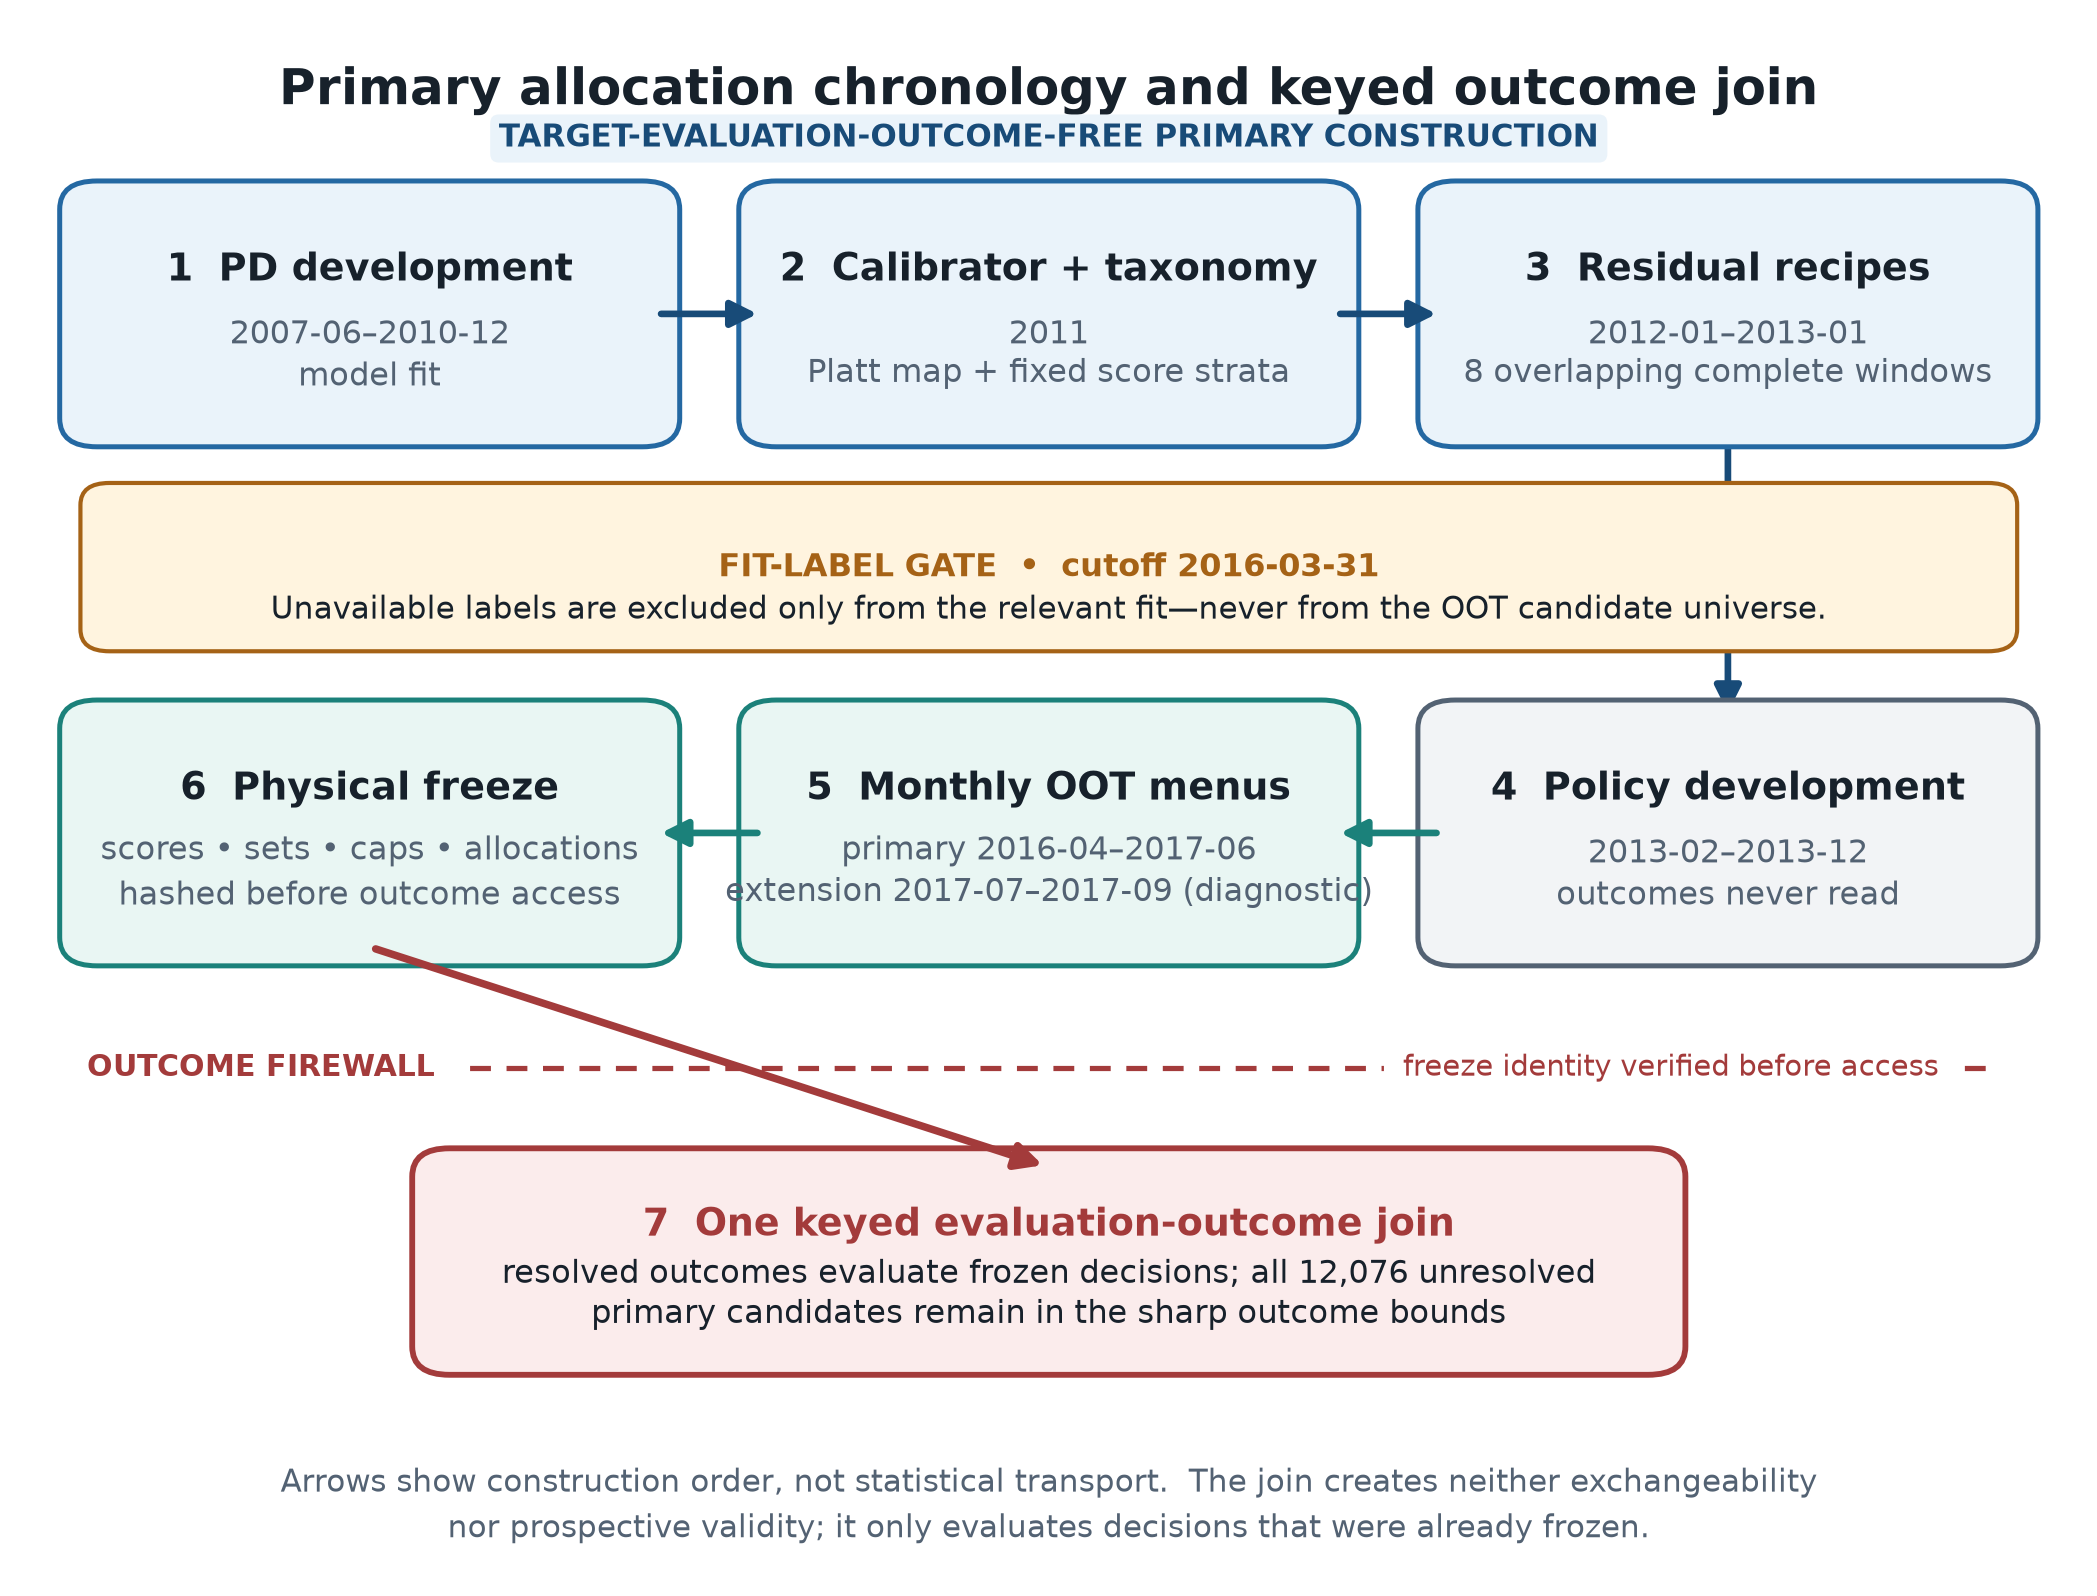
\includegraphics[width=1\linewidth,height=\textheight,keepaspectratio,alt={Primary allocation chronology from PD development through calibration, residual fitting, outcome-free policy construction, a phase-specific physical freeze, and a later keyed target-evaluation-outcome join.}]{../../reports/crpto/figures/crpto_ijds_information_boundary.png}

}

\caption{\label{fig-information-boundary}Primary allocation chronology
and keyed outcome join. Arrows show construction order, not statistical
transport. Unavailable fitting labels are excluded only from the
relevant fit; outcome availability never filters the OOT candidate
universe. In this primary allocation lineage, the final keyed join
evaluates already frozen decisions while retaining all 12,076 unresolved
primary candidates in sharp bounds; it supplies no exchangeability or
prospective validity.}

\end{figure}%

\subsection{Information boundary}\label{information-boundary}

As Figure~\ref{fig-information-boundary} makes explicit, two ID-keyed
panels enforce the boundary for the primary allocation lineage. The
decision panel admits only dated origination and contractual variables,
scores, prediction sets, and strata; the administrative-outcome panel is
joined one-to-one only after allocations are frozen. This separation
makes the timing claim testable but creates no statistical guarantee.
Retrospective sensitivities that rescan raw chunks enforce logical
target-outcome nonuse after filtering rather than claiming the same
phase-specific physical lockbox.

Label-dependent fitting is additionally restricted by an information
cutoff of March 31, 2016. A Fully Paid label becomes available at the
month-end of its last payment; a Charged Off label is conservatively
dated six calendar months after that month-end. Retained fitting-label
shares exceed 99\% in every block and residual month; unavailable labels
are excluded from fitting, not candidacy. SHA-256-locked freezes contain
all scores, recipes, allocations, and comparator tracks before the
outcome join. Reversed-ID and independent-solver checks audit
extreme-point allocations. The resulting 48 two-ruler cells are six
tracks viewed through eight overlapping recipes, not replications;
Online Supplement Appendix F records all counts, hashes, and replay
contracts.

This rule makes the chronology substantive rather than cosmetic. The
2012-- January 2013 residual windows are the latest declared cohorts
that meet the greater-than-99\% label-retention gate by March 31, 2016,
whereas primary scoring begins in April 2016. The target class
prevalence therefore was not available from resolved target outcomes
when the thresholds and allocations were frozen.

\subsection{Identification safeguards}\label{identification-safeguards}

The reusable audit has five stages: define status-independent monthly
menus and dated label availability; fit scores, taxonomies, and residual
recipes without evaluation outcomes; specify comparator rulers, solve
and persist the policy grid; join one keyed outcome panel and compute
candidate and paired-policy identification bounds; and report every
audited dimension. Within the frozen replay, this order prevents outcome
filtering, future-menu look-ahead, payoff mismatch, and result-dependent
comparator choice. It cannot undo prior inspection, create
preregistration, restore exchangeability, identify lifetime cash flows,
or extend the evaluated grid to universal support. Online Supplement
Appendices A and G give the full audit map and boundaries.

\section{Method}\label{sec-method}

The paper uses one conceptual map throughout: raw prediction,
Platt-scaled score, residual threshold and binary set, continuous
embedding, LP coefficient and constraint, allocation, and target-outcome
estimand. These are noninterchangeable objects. Let
\(q_{\mathrm{raw},i}\) be the uncalibrated CatBoost probability and
\(h_c\) one of the four frozen score maps. The calibrator sensitivity
audits

\[
q_{\mathrm{raw},i}\longrightarrow p_i^{(c)}
=h_c(q_{\mathrm{raw},i})
\]

through the binary-set layer only. The optimization path fixes \(c\) to
the active Platt map. For one frozen score stratum \(\mathcal C_g\) on
that primary path,

\[
\{(p_j,Y_j):j\in\mathcal C_g\}\longrightarrow c_g,\qquad
(p_i,c_{g(i)})\longrightarrow(\ell_i,u_i),
\]

\[
\begin{aligned}
(\ell_i,u_i)&\longrightarrow S_i=[\ell_i,u_i]\cap\{0,1\},\\
(p_i,u_i)&\longrightarrow q_i(\gamma)=p_i+\gamma(u_i-p_i),\\
q(\gamma)&\longrightarrow \mathcal A^*\!\left(q(\gamma)\right)
\longrightarrow a^{\mathrm{fr}}\!\left(q(\gamma)\right)
\longrightarrow M\!\left(a^{\mathrm{fr}},Y\right).
\end{aligned}
\]

Here \(\mathcal A^*(q)\) is the possibly set-valued optimal-allocation
set, \(a^{\mathrm{fr}}(q)\in\mathcal A^*(q)\) is the frozen solver
output, and \(M\) is a declared target-outcome functional.

\textbf{Construction map and non-implications.} The fork is essential:
\(S_i\) records boundary contact but leaves the subunit value of
\(u_i\), while \(Y\) enters \(M\) only at the keyed evaluation join.
Each arrow specifies how CRPTO builds an object; it is not an
inheritance arrow for validity. Score calibration cannot establish
residual exchangeability, and preserving every \(S_i\) can still change
portfolio ordering, and candidate-set validity would not by itself
become selected- or exposure-weighted funded-set validity. Later
sections audit each handoff separately.

\subsection{Platt-scaled default score and credit-risk
controls}\label{platt-scaled-default-score-and-credit-risk-controls}

The primary model is a protocol-fixed CatBoost classifier
\citep{prokhorenkova2018catboost} on 29 numeric and nine categorical
origination-time features, followed by a separate 2011 logistic Platt
map \citep{platt2000}. It is not tuned against downstream or OOT
outcomes. Four coverage-only controls change model class or information:
numeric logistic regression, domain-constrained monotonic CatBoost, a
platform-signal WOE/IV scorecard, and a pricing-excluded application
WOE/IV scorecard \citep{navaspalencia2020}. Each receives its own Platt
map and 2011 score taxonomy; only primary CatBoost enters optimization.
These are specification controls, not a leaderboard, and the primary
model is fixed by protocol rather than chosen: a control that attains
better OOT discrimination is not selected, because selecting it would be
the outcome-dependent choice this design exists to avoid.

Within each frozen learner specification, Platt scaling has a
deliberately narrow role: it is a scalar map fitted once on the separate
2011 block and then frozen. Its use is not a claim that Platt is the
best calibrator. A separately tagged retrospective sensitivity freezes
four maps of the same primary CatBoost base output on the same 14,077
availability-safe 2011 labels: the active Platt map (reused without
refitting), increasing isotonic regression with clipped out-of-domain
predictions \citep{zadrozny2002}, beta calibration with the \texttt{abm}
parameterization \citep{kull2017}, and inductive Venn--Abers prediction
\citep{vovk2014}. The active Platt edges are transformed exactly to the
uncalibrated-probability \(q_{\mathrm{raw}}\) scale, yielding one common
five-group taxonomy with zero assignment changes; method-specific ties
cannot change group membership because, to isolate the score map, we do
not rebin by method. For each frozen map, Phase A fits five-stratum
residual recipes in all eight windows; all four methods, the pooled
panel, and all five common strata are reported. No CatBoost model is
refitted.

Venn--Abers returns a multiprobabilistic pair \((p_{i0},p_{i1})\). The
declared point score is the standard positive-class scalarization

\[
p_i^\prime=\frac{p_{i1}}{1-p_{i0}+p_{i1}}.
\]

The runner retains and checks the pair, but \(p_i^\prime\) lacks its
multiprobability guarantee and is neither a latent-PD interval nor a
validated portfolio coefficient. Same-sample 2011 fit diagnostics are
descriptive only. Phase B evaluates 192 method--window--scope cells and
all 288 unordered pairwise cells using one loan-wise unresolved-label
completion per contrast. It performs no optimization and selects no
calibrator, window, stratum, efficiency result, or pairwise contrast.
Thus neither the comparison nor any method name repairs temporal
nonexchangeability, unavailable outcomes, or selection into funded
exposure. Generalized Venn predictors strengthen the case for keeping
the genuinely set-valued predictive object distinct from a scalar
summary \citep{vanderlaan2025generalized_venn}; they do not validate
this inductive Venn--Abers predictor (IVAP) scalarization or make it a
conformal optimization coefficient.

The raw-data contract predeclares mappings for structurally missing
delinquency recency and sparsely recorded bankruptcy count, and a frozen
sensitivity compares that sentinel convention with explicit indicators
and native nullable values. It covers those two fields rather than every
incomplete predictor and selects no encoding or missingness mechanism,
and it is a deterministic encoding comparison rather than a conformal
treatment of missingness \citep{zaffran2023missing}. Online Supplement
Appendix B gives features, hyperparameters, mappings, fit diagnostics,
and WOE/IV controls.

\subsection{Score-Mondrian binary prediction sets and continuous
interval
embedding}\label{score-mondrian-binary-prediction-sets-and-continuous-interval-embedding}

Let \(Y_i\in\{0,1\}\) denote terminal default and \(p_i\) the
Platt-scaled score. Write \(\widehat p_i(1)=p_i\) and
\(\widehat p_i(0)=1-p_i\). For either candidate label \(y\in\{0,1\}\),
the absolute-residual score is the standard probability-complement
classification score,

\begin{equation}\protect\phantomsection\label{eq-binary-nonconformity}{
s_i(y)=|y-p_i|=1-\widehat p_i(y).
}\end{equation}

Thresholding this score yields the same binary set form as
least-ambiguous set-valued classification \citep{sadinle2019lac}. This
algebraic equivalence cannot transfer oracle expected-size optimality to
estimated Platt scores or to the temporal, score-stratified construction
used here.

Five groups are fixed from 2011 score quantiles, without residual-window
labels; extreme strata are open-ended so every later score is retained.
Conditioning a split-conformal threshold on a frozen category in this
way is the Mondrian construction
\citep{vovk2003mondrian, vovk2012conditional}; here the category is the
outcome-free score stratum, not the label. Label-conditional calibration
is a standard alternative for severe class imbalance \citep{ding2023};
we report it retrospectively as a sensitivity, not as a proved repair
for temporal nonexchangeability or as the active recipe. The
specification reports all eight consecutive six-month windows beginning
January--August 2012. For \(n_g\) observations and target
\(\alpha=0.10\), the split-conformal rank is

\begin{equation}\protect\phantomsection\label{eq-rank}{
k_g=\left\lceil(n_g+1)(1-\alpha)\right\rceil,
}\end{equation}

and \(c_g\) is the \(k_g\)-th smallest residual in ascending order. If
\(k_g=n_g+1\), the active binary implementation uses the equivalent cap
\(c_g=1\); every binary candidate label is then included, just as under
\(+\infty\). The taxonomy, group assignment, and score map must remain
frozen independently of the calibration and target outcomes. A future
score assigned to group \(g(i)\) receives

\begin{equation}\protect\phantomsection\label{eq-interval}{
[\ell_i,u_i]=
\left[\max\{0,p_i-c_{g(i)}\},\min\{1,p_i+c_{g(i)}\}\right].
}\end{equation}

The same threshold defines the canonical binary classification set

\begin{equation}\protect\phantomsection\label{eq-binary-set}{
S_i=\left\{y\in\{0,1\}:|y-p_i|\le c_{g(i)}\right\}
   =[\ell_i,u_i]\cap\{0,1\}.
}\end{equation}

If the \(n_g\) calibration nonconformity scores and the future
nonconformity score are exchangeable within the frozen stratum, the
inclusive rule satisfies
\(\Pr\{Y_{\mathrm{new}}\in S(X_{\mathrm{new}})\mid G_{\mathrm{new}}=g\}\ge
1-\alpha\), marginally over calibration and that future unit
\citep{vovk2005, angelopoulos2023}. CRPTO makes no assertion that this
temporal exchangeability condition holds.

Thus coverage of \(S_i\) and \([\ell_i,u_i]\) coincides for binary
\(Y_i\), but the interval is a continuous design embedding, generally
not the convex hull of \(S_i\), and \(u_i\) is the downstream score
input. Two loans can therefore have the same binary set but different
\(u_i\); no coverage property gives \(u_i\) a probabilistic magnitude or
orders it within that fixed set. Neither object is a confidence interval
for latent PD or a funded-set guarantee. No outcome-dependent widening
or taxonomy adaptation enters a recipe. The closed 1-, 2-, 5-, and
10-group grid is reported for CatBoost and numeric logistic; monotonic
CatBoost and the two WOE controls retain their own five-group recipes.
All are coverage diagnostics, not a selection grid.

The formal set-to-embedding nonidentification lemma, its complete
compatible fibre, and the exact decision-invariance boundary are stated
together in Section~\ref{sec-theory}.

The four possible binary sets are \(\varnothing\), \(\{0\}\), \(\{1\}\),
and \(\{0,1\}\), with candidate shares \(e,z,o,b\) summing to one. Mean
set cardinality is then \(\operatorname{AvgC}=1-e+b\) and the singleton
share is \(\operatorname{OneC}=1-e-b\); both are bookkeeping identities
rather than results. Reporting \(e\) and \(b\) separately prevents an
average cardinality from hiding never-covered empty sets or
uninformative two-label sets, and neither metric is a coverage
guarantee.

The baseline above is Mondrian only with respect to the outcome-free
score stratum; it uses one marginal residual threshold within each
stratum. The retrospective label-Mondrian sensitivity instead freezes,
for each label \(y\) in each stratum \(g\),

\begin{equation}\protect\phantomsection\label{eq-label-rank}{
k_{g,y}=\left\lceil(n_{g,y}+1)(1-\alpha)\right\rceil,
\qquad q_{g,y}=R^{(k_{g,y})}_{g,y},
}\end{equation}

where residuals are ordered ascending and the binary implementation uses
the equivalent cap \(q_{g,y}=1\) when \(k_{g,y}=n_{g,y}+1\). Before the
OOT outcome join, it then constructs

\begin{equation}\protect\phantomsection\label{eq-label-mondrian}{
S_i^{\mathrm{LM}}=
\{0:p_i\le q_{g(i),0}\}\cup
\{1:1-p_i\le q_{g(i),1}\}.
}\end{equation}

The set need not be symmetric around \(p_i\). Class-specific coverage is
a ratio rather than an additive functional, so its sharp bounds assign
unresolved candidates according to whether the class is contained in the
set. Bounds on the class gap give each unresolved loan one label shared
by both class ratios within each bound endpoint; only completions with
positive denominators for both classes are admissible. Both resolved
classes are nonempty in every active cell, so this condition removes no
reported completion. Subtracting separately optimized intervals is not
sharp. Online Supplement Appendix B.4.2 gives the ratio formulas and all
40/200/400 rows. They are identification diagnostics, not tests.

\begin{longtable}[]{@{}
  >{\raggedright\arraybackslash}p{(\linewidth - 4\tabcolsep) * \real{0.3333}}
  >{\raggedright\arraybackslash}p{(\linewidth - 4\tabcolsep) * \real{0.3333}}
  >{\raggedright\arraybackslash}p{(\linewidth - 4\tabcolsep) * \real{0.3333}}@{}}
\caption{Score-Mondrian and label-Mondrian answer different conditional
questions and have different roles in the
audit.}\label{tbl-mondrian-roles}\tabularnewline
\toprule\noalign{}
\begin{minipage}[b]{\linewidth}\raggedright
Design dimension
\end{minipage} & \begin{minipage}[b]{\linewidth}\raggedright
Active score-Mondrian recipe
\end{minipage} & \begin{minipage}[b]{\linewidth}\raggedright
Retrospective label-Mondrian sensitivity
\end{minipage} \\
\midrule\noalign{}
\endfirsthead
\toprule\noalign{}
\begin{minipage}[b]{\linewidth}\raggedright
Design dimension
\end{minipage} & \begin{minipage}[b]{\linewidth}\raggedright
Active score-Mondrian recipe
\end{minipage} & \begin{minipage}[b]{\linewidth}\raggedright
Retrospective label-Mondrian sensitivity
\end{minipage} \\
\midrule\noalign{}
\endhead
\bottomrule\noalign{}
\endlastfoot
Frozen category & One outcome-free 2011 score stratum \(g\) & The same
score stratum crossed with candidate label \(y\) \\
Thresholds & One residual quantile pooled over labels within each fixed
score stratum & Separate \(q_{g,0}\) and \(q_{g,1}\) \\
Binary set & Symmetric absolute-residual rule, then intersection with
\(\{0,1\}\) & Include each label against its own threshold; the set need
not be symmetric around \(p_i\) \\
Validity contract & Exchangeability within each fixed score stratum &
Exchangeability within each fixed score-stratum--label category \\
Role in CRPTO & Primary score-Mondrian recipe; only its CatBoost score
enters optimization & Retrospective coverage sensitivity over all
reported cells; never enters the optimizer \\
Shared boundary & No temporal-transport or funded-set validity follows &
No repair, fairness conclusion, or selected method follows \\
\end{longtable}

For binary \(Y\), miscoverage has the useful identity

\begin{equation}\protect\phantomsection\label{eq-binary-miss}{
m_i=\mathbf 1\{Y_i\notin S_i\}
   =\mathbf 1\{Y_i=0,\ell_i>0\}+
    \mathbf 1\{Y_i=1,u_i<1\}.
}\end{equation}

Thus a default is counted as covered whenever \(u_i=1\), even though
such an upper bound endpoint offers little discrimination to the
optimizer. Conversely, a narrow low-score interval with \(u_i<1\) misses
every realized default. This geometry is central to interpreting the
funded-set miscoverage diagnostic, but it cannot establish funded-set
conformal validity.

\subsection{Joint-block combined-rank reference
diagnostic}\label{joint-block-combined-rank-reference-diagnostic}

The finite-archive completion bounds in Section~\ref{sec-theory} answer
what coverage is attainable; they do not test exchangeability. We
therefore define a separate rank-reference diagnostic. In frozen stratum
\(g\), let \(n_g\) be the calibration size,
\(r_g=\lceil(n_g+1)(1-\alpha)\rceil\), and \(m_g\) the target size.
Conditional on the frozen taxonomy and the realized stratum memberships
and counts \((n_g,m_g)\), a strict miss is a target residual \(R>c_g\).
Under joint continuous exchangeability of the \(n_g+m_g\) calibration
and target residual scores as one block, assume \(r_g\le n_g\), as in
every evaluated stratum. If instead \(r_g=n_g+1\), the standard fitted
threshold is \(+\infty\) (stored as cap 1 for residuals in \([0,1]\))
and \(M_g=0\) deterministically; the distribution below is not invoked.
For \(r_g\le n_g\), the number of strict target misses has the exact
combined-rank law

\begin{equation}\protect\phantomsection\label{eq-rank-reference}{
M_g\sim\operatorname{BetaBinomial}
\left(m_g,n_g+1-r_g,r_g\right),
\qquad
E(M_g/m_g)=\frac{n_g+1-r_g}{n_g+1}.
}\end{equation}

Uniform combined ranks give this law without score independence. Its
expected miss rate is the displayed finite-sample fraction, not
necessarily 0.10. The null is stronger than
calibration-plus-one-future-point exchangeability, so a flag may reflect
target-block dependence or heterogeneity without refuting the usual
marginal guarantee.

The tie-free law is the finite-batch empirical-coverage result of
\citet{marques2025universal}, written for the complementary strict-miss
count. Lexicographic iid auxiliaries make combined ranks continuous
while leaving the reported sets deterministic. Because the strict-miss
count cannot exceed its augmented counterpart, the Beta--Binomial upper
tail is conservative. The observed absence of threshold ties cannot
prove continuity.

Minimizing attainable strict misses gives the supremum upper-tail
p-value over all unrestricted binary completions. The locked calculation
uses Bonferroni across five strata and Holm \citep{holm1979} across 40
learner-window intersections. The shared calibration block induces
dependent conformal p-values rather than a product law
\citep{gazin2024transductive}. Training- or calibration-conditional
coverage is a distinct target studied through probably approximately
correct (PAC) or high-probability guarantees under stronger sampling
contracts
\citep{vovk2012conditional, bian2023training_conditional, duchi2025sampleconditional}.
We retain the batch rank reference because its finite-batch null is
explicit and legible. Holm already allows arbitrary dependence among
valid p-values; changing the evidence currency would not repair
inspection of the family or flag pattern. Because an exploratory
implementation and pattern were inspected before the diagnostic was
locked, these are nominal reporting thresholds, not post-selection
familywise error rate (FWER) control. They do not cover the 200 strata
or any sensitivity. A flag identifies neither theorem failure nor
mechanism; a nonflag establishes neither exchangeability nor
transportability.

\subsection{Model-implied plug-in objective and status-indexed payoff
proxy}\label{model-implied-plug-in-objective-and-status-indexed-payoff-proxy}

For contractual annual rate \(r_i\) and fixed loss given default
\(\lambda=0.45\), define the per-dollar status-indexed standardized
payoff proxy

\begin{equation}\protect\phantomsection\label{eq-status-payoff}{
\pi_i(Y_i)=(1-Y_i)r_i-Y_i\lambda,
}\end{equation}

with model-implied plug-in objective coefficient

\begin{equation}\protect\phantomsection\label{eq-expected-payoff}{
\bar\pi_i=(1-p_i)r_i-p_i\lambda.
}\end{equation}

This coefficient equals the conditional expectation of the proxy only if
\(p_i\) equals the conditional default probability. We use it as a
model-implied plug-in objective and evaluate the corresponding
status-indexed proxy, not as proof of conditional calibration. The pair
intentionally omits payment timing, principal amortization, prepayment,
fees, recoveries, and discounting. We therefore do not call the payoff
proxy profit, cash-flow return, NPV, welfare, or IRR. In particular, the
annual rate and the 36-month terminal label do not share a cash-flow
time scale; their relative coefficient is a declared decision-score
normalization, not accumulated contractual interest.

In month \(t\), let \(a_{it}\) be dollar exposure to loan \(i\), bounded
by its listed amount \(A_i\). For a policy \((\tau,\gamma)\), the LP is

\begin{equation}\protect\phantomsection\label{eq-lp}{
\begin{aligned}
\max_{a_{it}}\quad & \sum_{i\in\mathcal I_t}a_{it}\bar\pi_i \\
\text{s.t.}\quad
& \sum_i a_{it}=B, \\
& \sum_i a_{it}q_i(\gamma)\le \tau B, \\
& \sum_{i:\,purpose_i=k}a_{it}\le 0.25B \quad\forall k,\\
& 0\le a_{it}\le A_i,
\end{aligned}
}\end{equation}

where \(B=\$1\) million in every month. The point-score baseline sets
\(\gamma=0\). The objective is identical across policies, so differences
arise from the risk score and the loans made feasible by it. The LP
permits fractional dollar exposure. A separately frozen implementation
diagnostic floors each positive exposure to a USD 25 lot and holds the
residual as cash; it performs no reoptimization or define an
integer-policy estimand.

\subsection{Common-frontier rulers and supporting comparator
audit}\label{common-frontier-rulers-and-supporting-comparator-audit}

Let \(\mathcal A_t\) contain the budget, loan-bound, and purpose
constraints in Equation~\ref{eq-lp}, let \(v_i=\bar\pi_i\), and let
\(s_i(\gamma)=q_i(\gamma)\) for \(\gamma\in\{0,0.25,0.50,0.75,1\}\). For
every month and score, define the minimum funded score, the common
unconstrained plug-in optimum, and the score of that optimum as

\begin{equation}\protect\phantomsection\label{eq-ruler-anchors}{
m_{\gamma t}=B^{-1}\min_{a\in\mathcal A_t}s(\gamma)^\top a,
\quad z_t^*=\max_{a\in\mathcal A_t}v^\top a,
\quad o_{\gamma t}=B^{-1}s(\gamma)^\top a_t^*.
}\end{equation}

The normalized anchor is accepted only after an objective-tie audit. For
each score, we minimize and maximize funded score over the USD
\(10^{-7}\) plug-in-optimal face; any range above \(10^{-8}\) stops the
run rather than allowing an unresolved objective tie to define
\(o_{\gamma t}\).

The primary \textbf{objective-matched ruler} compares scores at a common
plug-in opportunity cost. To make ties explicit, let
\(z^{\min}_{\gamma t}\) be the objective-efficient point on the
minimum-score face, that is the maximum of \(v^\top a\) over
\(a\in\mathcal A_t\) with \(s(\gamma)^\top a=B m_{\gamma t}\) at the
registered solver tolerances, and set
\(z_t^L=\max_\gamma z^{\min}_{\gamma t}\). At
\(\rho\in\{0.25,0.50,0.75\}\), every score solves

\begin{equation}\protect\phantomsection\label{eq-objective-ruler}{
\min_{a\in\mathcal A_t}s(\gamma)^\top a
\quad\text{s.t.}\quad
v^\top a\ge z_t^L+\rho(z_t^*-z_t^L).
}\end{equation}

The shared floor is a model-implied objective, not true expected return.
The secondary \textbf{normalized-score ruler} instead sets

\begin{equation}\protect\phantomsection\label{eq-normalized-ruler}{
c_{\gamma t}(\eta)=m_{\gamma t}
  +\eta(o_{\gamma t}-m_{\gamma t}),\qquad
\eta\in\{0.25,0.50,0.75\},
}\end{equation}

and maximizes \(v^\top a\) subject to
\(s(\gamma)^\top a\le Bc_{\gamma t}(\eta)\). Equal \(\eta\) is invariant
to a positive affine rescaling of a score, but it is not equal default
risk, objective sacrifice, or operational tolerance. At coordinate one
both rulers reach the verified common plug-in objective value, so only
that objective-value contrast is structurally null unless the common
optimizer is unique or reused by definition. The empirical diagnostic is
therefore the reported three-coordinate interior grid, not a
continuous-frontier claim.

For each ruler and coordinate, the frozen contrast is \(\gamma=1\) minus
\(\gamma=0\). Interior gamma values verify the path but cannot be
selected as winners. Every allocation is outcome-free; unresolved
outcomes enter only through the common-outcome bounds after the freeze.

A supporting audit compares the grid with same-cap C0,
development-supported C1, funded-point-moment C2, and 3,067 registered
point caps over the development and {[}0.05,0.12{]} supports. C2 is an
executable two-solve decomposition comparator. It is not a selected
operating policy, an independently specified baseline, or a matched
feasible-set counterfactual. Online Supplement Appendix C defines every
comparator. No evaluation outcome chooses a track, although this
within-lineage isolation cannot imply that the global analysis family
preceded archive inspection.

\section{Audit Theory and Estimands}\label{sec-theory}

The theory is organized into two suites. Prediction geometry separates
binary thresholds, crossed-band coverage, set-to-embedding
nonidentification, and completion bounds. Decision geometry then
characterizes feasible-order equivalence, ruler and comparator
consequences, set-native degeneracy, and the registered-support
boundary. None of the statements assumes funded-set conformal validity
or makes one ruler uniquely correct. Online Supplement Appendix B.5 and
Online Supplement Appendix D contain the derivations and proofs.

\subsection{Prediction geometry and partial
identification}\label{prediction-geometry-and-partial-identification}

\subsubsection{Exact binary threshold and crossed-band
geometry}\label{exact-binary-threshold-and-crossed-band-geometry}

Because \(s_i(Y_i)=p_i\) when \(Y_i=0\) and \(1-p_i\) when \(Y_i=1\),
the calibration residuals of a stratum are the multiset sum of two
mirror samples, so the fitted threshold is an order statistic of that
union and its regime is fixed by a count rather than by a population
idealization.

\textbf{Proposition 1 (exact binary threshold geometry).} In a frozen
stratum with calibration scores \(p_i\in[0,1]\), default count \(D\),
and rank \(k\le n\) from Equation~\ref{eq-rank}, let
\(R=\{\!\{p_i:Y_i=0\}\!\}\uplus\{\!\{1-p_i:Y_i=1\}\!\}\). Then
\(c=R_{(k)}\); with \(A=\#\{Y_i=0,p_i<1/2\}\) and
\(B=\#\{Y_i=1,p_i>1/2\}\), \(c<1/2\) if and only if \(A+B\ge k\); and
\(n-k=\lfloor\alpha(n+1)\rfloor-1\) exactly. If in addition
\(\max_i p_i<1/2\), then \(A=n-D\) and \(B=0\), so \(c<1/2\) if and only
if the \emph{phase margin} \(m=D-(n-k)\) is nonpositive. When both
calibration classes are nonempty, under the weaker no-interleaving
condition below, when \(m\le0\) the threshold is the \(k\)-th smallest
nondefault score; when \(m\ge1\) it is \(1-p^1_{[m]}\), where
\(p^1_{[m]}\) is the \(m\)-th largest default score. Thus \(m=0\) gives
the maximum nondefault score and \(m=1\) gives one minus the maximum
default score, but those values belong to their respective calibration
blocks and are not coupled through a common pair of maxima.

With both calibration classes nonempty, the weaker condition
\(\max_{Y_i=0}p_i+\max_{Y_i=1}p_i<1\) determines only which mirror
sample supplies \(c\) while leaving whether \(c<1/2\) unresolved.
Statements about a target unit need their own support condition:
covering \(Y=1\) requires \(p\ge1-c\). Thus a stratum misses every
realized target default exactly when none has \(p\ge1-c\). On a finite
candidate panel, \(\max_i p_i<1-c\) over all target candidates is an
outcome-free sufficient condition, not a necessary one.

\textbf{Lemma 1 (exact coverage-band identity).} By
Equation~\ref{eq-binary-miss}, stratum coverage at threshold \(c\) is
\((1-\pi_t)\Pr_t(p\le c\mid Y=0)+\pi_t\Pr_t(p\ge1-c\mid Y=1)\).
Therefore, for any fixed target distribution and \(0\le c_L<c_H\le1\),

\begin{equation}\protect\phantomsection\label{eq-coverage-band}{
\begin{aligned}
\operatorname{Cov}(c_H)-\operatorname{Cov}(c_L)
={}&\Pr_t(Y=0,c_L<p\le c_H)\\
 &+\Pr_t(Y=1,1-c_H\le p<1-c_L).
\end{aligned}
}\end{equation}

Equivalently, the two terms are weighted by \((1-\pi_t)\) and \(\pi_t\)
after conditioning on the class. The identity is exact and nonnegative:
coverage can change only through target mass in the two crossed score
bands. It does not imply continuity or make the change small
universally; atoms can produce an order-one change even when scores
vary. For unresolved target outcomes, sharp bounds follow loan by loan
from the minimum and maximum, over \(y\in\{0,1\}\), of the difference
between the two coverage indicators. Online Supplement B.5 proves both
statements.

\textbf{Corollary 1 (low-regime coverage ceiling).} In a stratum with
\(c<1/2\), coverage on one fixed target distribution satisfies

\begin{equation}\protect\phantomsection\label{eq-low-regime-coverage-ceiling}{
\operatorname{Cov}_t
\le 1-\pi_t+\pi_t\Pr_t(p\ge1-c\mid Y=1).
}\end{equation}

If, in addition, every target score in the stratum is below \(1-c\),
then \(\operatorname{Cov}_t\le1-\pi_t\): the stratum can cover at most
the nondefault share. The target-support condition is sufficient, not
necessary. The phase condition fixes \(c<1/2\) from calibration data,
while target support determines the remaining default-coverage term.
This ceiling concerns one fixed target distribution; it is not a
transport statement or a mechanism claim.

The protocol-locked and hash-verified common-panel replay applies this
identity to every adjacent pair: five learners by five fixed score
strata by seven transitions, or 175 contrasts, plus 35 learner-level
aggregates. It recomputes all 200 calibration thresholds from their
frozen order statistics. For unresolved loan \(i\), it uses the same
loan-specific label under both thresholds, so the sharp bound endpoints
add \(\min_y d_i(y)\) and \(\max_y d_i(y)\) loan by loan. Subtracting
two separately extremized coverage intervals would answer a different,
incoherent question.

\subsubsection{Set-to-embedding
nonidentification}\label{set-to-embedding-nonidentification}

\textbf{Lemma 2 (nonidentification of the continuous decision
coefficient).} For any \(0\le\ell_i\le u_i\le1\),

\[
\begin{array}{c|c}
S_i=[\ell_i,u_i]\cap\{0,1\} & \text{necessary and sufficient bound condition}\\
\hline
\varnothing & \ell_i>0,\ u_i<1\\
\{0\} & \ell_i=0,\ u_i<1\\
\{1\} & \ell_i>0,\ u_i=1\\
\{0,1\} & \ell_i=0,\ u_i=1.
\end{array}
\]

Consequently, when \(1\notin S_i\), binary-set membership and every
coverage event identify only \(u_i<1\), not its continuous magnitude.
For the active embedding, the outcome-free family

\begin{equation}\protect\phantomsection\label{eq-set-preserving-embedding}{
u_i^{(\theta)}=
\begin{cases}
(1-\theta)u_i+\theta p_i,&1\notin S_i,\\
1,&1\in S_i,
\end{cases}\qquad 0\le\theta\le1
}\end{equation}

keeps \(\ell_i\le p_i\le u_i^{(\theta)}\le u_i\), preserves \(S_i\) loan
by loan, and therefore preserves binary-set coverage. It can
nevertheless change the LP coefficient
\((1-\gamma)p_i+\gamma u_i^{(\theta)}\). Conformal validity alone
therefore cannot choose an embedding, prove that an allocation changes,
or order its decision consequences. The complete finite sensitivity
reported below is separate empirical evidence; its allocation changes
cannot be inferred from this lemma alone.

The complete compatible fibre makes the information loss explicit. If
the continuous interval must contain \(p_i\) and \(0<\gamma\le1\), every
set-equivalent coefficient lies in

\begin{equation}\protect\phantomsection\label{eq-compatible-embedding-fibre}{
q_i\in
\begin{cases}
\{p_i+\gamma(1-p_i)\},&1\in S_i,\\
[p_i,p_i+\gamma(1-p_i)),&1\notin S_i.
\end{cases}
}\end{equation}

At \(\gamma=0\) the coefficient is simply \(p_i\). Under a rectangular
ambiguity set over these fibres and nonnegative allocations, the
worst-case coefficient has supremum \(p_i+\gamma(1-p_i)\) for every
loan. Thus at \(\gamma=1\) a full-budget score cap below one is
infeasible; with optional cash the same cap reduces to a bound on total
invested capital and no longer distinguishes loans. For sets without
label one this is a supremum over the open upper bound endpoint, not an
attained maximum. Extra cross-loan structure or an exogenous upper bound
below one would define a different model. Naively robustifying the
unidentified continuous lifting therefore fails to produce an
informative set-native credit ordering.

For the active contraction,

\begin{equation}\protect\phantomsection\label{eq-active-embedding-score-change}{
q_i^{(\theta)}-q_i^{(0)}
=-\gamma\theta c_{g(i)}\mathbf 1\{1\notin S_i\}.
}\end{equation}

Set preservation places no positive-affine restriction on this vector
over feasible allocation differences. Proposition 2 states the exact
decision-invariance condition.

\subsubsection{Binary completion bounds}\label{binary-completion-bounds}

\textbf{Lemma 3 (sharp outcome-free bounds for a fixed allocation).} Fix
\(a_i\ge0\) with total funded exposure \(B_a=\sum_i a_i>0\). Over
unrestricted loan-wise binary outcomes, exposure-weighted miscoverage
satisfies the sharp bounds

\begin{equation}\protect\phantomsection\label{eq-outcome-free-set-bounds}{
\frac{\sum_i a_i\mathbf 1\{S_i=\varnothing\}}{B_a}
\ \le\ \operatorname{MC}(a,Y)\ \le\
1-\frac{\sum_i a_i\mathbf 1\{S_i=\{0,1\}\}}{B_a}.
}\end{equation}

Empty sets miss both labels and full sets cover both; every singleton
can be made covered or missed independently, so both bound endpoints are
attainable. A positive lower bound endpoint alone is not a miss: if
\(u_i=1\), label one is covered. Likewise, \(\sum_i a_i1\{u_i=1\}/B_a\)
measures total-capital exposure capable of covering a positive label,
not conditional positive-class coverage. This lemma is fixed-allocation
set algebra, not funded-set conformal validity or an optimizer-direction
result.

For an unresolved loan, \(Y_i\) may be either 0 or 1. Default therefore
lies in \([0,1]\), payoff in \([-\lambda,r_i]\), and miscoverage in the
two attainable values implied by Equation~\ref{eq-binary-miss}.

Throughout the paper, a reported bracket \([T_L,T_U]\) for a finite
binary-completion problem denotes the sharp \emph{bound-endpoint hull}:
each bound endpoint is attained by an admissible joint completion. The
attainable identified set may be a finite or otherwise nonconvex subset
of that hull, so interior values are not asserted attainable. Sharpness
is cellwise unless joint attainability across cells is stated
explicitly.

\textbf{Lemma 4 (sharp common-outcome bounds and width).} Let \(U\)
index unrestricted outcomes and write an additive fixed-allocation
metric as \(T(Y)=C+\sum_{i\in U}g_i(Y_i)\). Then

\begin{equation}\protect\phantomsection\label{eq-sharp-bounds}{
T_L=C+\sum_{i\in U}\min_{y\in\{0,1\}}g_i(y),\qquad
T_U=C+\sum_{i\in U}\max_{y\in\{0,1\}}g_i(y)
}\end{equation}

are sharp because each bound endpoint is attained by a joint assignment
of all unresolved outcomes. This is partial identification under
unrestricted binary completion in the sense of
\citet{manski2003partial}, not a sampling confidence interval. The
unresolved outcomes here arise from an administrative availability rule
rather than from a decision, so this is the binary-completion problem
rather than the selective-labels and reject-inference problems described
in Related Work. The estimands are finite-archive coverage and
frozen-policy outcome functionals \citep{maiapolo2024partial_id_eval};
the design imputes no point labels.

For candidate coverage, resolved \(R\) retain observed miscoverage and
only unresolved \(U\) are completed. The sharp bound-endpoint hull is

\begin{equation}\protect\phantomsection\label{eq-sharp-coverage}{
\left[
1-\frac{1}{n}\left\{\sum_{i\in R}m_i(Y_i)+
\sum_{i\in U}\max_{y\in\{0,1\}}m_i(y)\right\},
1-\frac{1}{n}\left\{\sum_{i\in R}m_i(Y_i)+
\sum_{i\in U}\min_{y\in\{0,1\}}m_i(y)\right\}
\right].
}\end{equation}

For paired policies, marginal-interval subtraction is not sharp. On the
union of funded IDs, retain signed exposure differences and assign each
unresolved \(Y_i\) once to both policies. For contribution \(d_i(Y_i)\),

\begin{equation}\protect\phantomsection\label{eq-identification-width}{
T_U-T_L=\sum_{i\in U}\left|d_i(1)-d_i(0)\right|.
}\end{equation}

For normalized exposure difference \(\delta_i^w=a_i^A/N_A-a_i^B/N_B\),
payoff-rate, default-rate, and miscoverage-rate widths are respectively
\(\sum_U|\delta_i^w|(r_i+\lambda)\), \(\sum_U|\delta_i^w|\), and
\(\sum_U|\delta_i^w||m_i(1)-m_i(0)|\). Here \(N_A=N_B=B\), including the
floor-with-cash diagnostic. The corresponding dollar-payoff width is
\(\sum_U|a_i^A-a_i^B|(r_i+\lambda)\). The simplified miscoverage
expression assumes both policies are evaluated with the same frozen
prediction-set map \(m_i(y)\), as in the active comparisons. With
policy-specific sets, the general identity remains valid after defining
\(d_i(y)=a_i^A m_i^A(y)/N_A-a_i^B m_i^B(y)/N_B\), but the simplified
factorization need not. Identification loss therefore depends on
exposure disagreement and set geometry, not merely the unresolved count.

\subsection{Decision geometry}\label{decision-geometry}

\subsubsection{Feasible-order
equivalence}\label{feasible-order-equivalence}

The next result is an elementary finite-dimensional linear-algebra
characterization of two linear functionals restricted to the span of
feasible allocation differences; it invokes neither parametric-LP
regularity nor optimizer uniqueness.

\textbf{Proposition 2 (feasible-difference score-order equivalence).}
Let \(\mathcal A\) be the fixed nonempty convex allocation set before
adding a score constraint and let
\(D=\operatorname{span}(\mathcal A-\mathcal A)\). Two score vectors
\(s\) and \(t\) induce the same weak order over every allocation in
\(\mathcal A\) if and only if

\begin{equation}\protect\phantomsection\label{eq-feasible-difference-equivalence}{
t=\kappa s+h,\qquad \kappa>0,\quad h\in D^\perp.
}\end{equation}

Equivalently, \(t^\top a=\kappa s^\top a+\delta\) throughout
\(\mathcal A\). If the affine hull is exactly the full-budget
hyperplane, this reduces to \(t=\kappa s+b\mathbf 1\). For the optimizer
statements that follow, the invoked optima are assumed to be attained,
as they are on the bounded CRPTO allocation polytope. Translated caps
then define the same feasible set; every objective-matched problem at a
common plug-in floor has the same complete argmin set; and normalized
coordinates define the same cap set when they use a common objective
anchor. Equality of binary sets or of the coordinatewise loan ranking is
insufficient for this condition. Its failure permits but cannot force a
decision change in one fixed cell, and one common solver-returned
allocation cannot establish equality of optimal faces. Online Supplement
D.2 gives the proof and counterexamples. As a related but different use
of the same geometry, Wei and Zhang characterize co-optimal linear
objectives over one common feasible set by common-normal-cone membership
\citep{wei2024adjustability}. CRPTO instead holds the objective fixed
while its score constraint can change the feasible set.

\textbf{Three-loan intuition.} Suppose a full budget is divided among
three loans. The score vectors \(s=(0,.6,1)\) and \(t=(0,.36,1)\) rank
the individual loans in the same order. Yet loan 2 has score \(.6\)
under \(s\), exceeding the \(.5\) score of an equal loan-1/loan-3
mixture, while under \(t\) its \(.36\) is below the mixture's \(.5\). A
ranking-preserving nonlinear transformation has therefore reversed a
portfolio comparison. Binary-set equality is weaker still: with
\(p=(.3,.1,.8)\) and thresholds \(c=(.3,.6,.3)\), both the original and
contracted embeddings induce \((\{0\},\{0\},\{1\})\), but their
continuous score vectors are \((.6,.7,1)\) and \((.3,.1,1)\) and can
choose different mixtures. Appendix D.2 gives the exact allocations. The
invariant must consequently be stated on feasible allocation
differences, not on loan ranks or set labels.

\subsubsection{Ruler and comparator
consequences}\label{ruler-and-comparator-consequences}

Let \(\mathcal F_s(\tau)\) denote the allocations satisfying
Equation~\ref{eq-lp} when the risk score is \(s\). All nonrisk
constraints and the objective are held fixed.

\textbf{Corollary 2 (what comparator matching preserves).} Suppose the
budget binds, \(\sum_i a_i=B\).

\begin{enumerate}
\def\labelenumi{\arabic{enumi}.}
\tightlist
\item
  If \(s_i=\kappa p_i+b\) with \(\kappa>0\), then
\end{enumerate}

\begin{equation}\protect\phantomsection\label{eq-affine-cap}{
\sum_i a_i s_i\le \tau_s B
\quad\Longleftrightarrow\quad
\sum_i a_i p_i\le \frac{\tau_s-b}{\kappa}B.
}\end{equation}

\begin{enumerate}
\def\labelenumi{\arabic{enumi}.}
\setcounter{enumi}{1}
\tightlist
\item
  If \(u_i\ge p_i\) and the same numerical cap is copied to
  \(q_i(\gamma)\), then
\end{enumerate}

\begin{equation}\protect\phantomsection\label{eq-feasible-nesting}{
\mathcal F_q(\tau)\subseteq\mathcal F_p(\tau).
}\end{equation}

\begin{enumerate}
\def\labelenumi{\arabic{enumi}.}
\setcounter{enumi}{2}
\tightlist
\item
  For \(\widetilde s=\kappa s+b\), the normalized ruler transforms as
  \(c_{\widetilde s}(\eta)=\kappa c_s(\eta)+b\), so
\end{enumerate}

\begin{equation}\protect\phantomsection\label{eq-normalized-invariance}{
\widetilde s^\top a\le Bc_{\widetilde s}(\eta)
\quad\Longleftrightarrow\quad
s^\top a\le Bc_s(\eta).
}\end{equation}

\begin{enumerate}
\def\labelenumi{\arabic{enumi}.}
\setcounter{enumi}{3}
\tightlist
\item
  Define \(V_p(c)=\max_{a\in\mathcal F_p(c)}\bar\pi^\top a\). If C2 sets
  \(c=(p^\top a^q)/B\) for a full-upper-score allocation \(a^q\), that
  allocation is feasible for the point-score LP and
\end{enumerate}

\begin{equation}\protect\phantomsection\label{eq-c2-dominance}{
V_p(c)\ge \bar\pi^\top a^q.
}\end{equation}

Parts 1 and 3 are exact invariances. Parts 2 and 4 mechanically order
feasible plug-in objectives, not realized payoff, default, or
miscoverage.

\subsubsection{Comparator-support
boundary}\label{comparator-support-boundary}

Let comparator \(j\) produce a sharp contrast interval \([L_j,U_j]\) for
a fixed full-upper-score policy and metric. For a declared finite set
\(\mathcal J\), define

\begin{equation}\protect\phantomsection\label{eq-multiverse}{
\mathcal I_{\mathcal J}=
\left[\min_{j\in\mathcal J}L_j,\max_{j\in\mathcal J}U_j\right].
}\end{equation}

The declared comparator sensitivity envelope \(\mathcal I_{\mathcal J}\)
summarizes bound endpoints over a named finite comparator set. A sign
survives only when the envelope lies strictly on one side of zero; this
is deterministic design sensitivity, not universal quantification over
baselines.

Supplemental Lemma 5 records a conditional endpoint-sufficiency fact:
within one fixed basis, a unique optimizer varies affinely with the cap,
so adverse sharp-bound extrema occur at that range's endpoints. Neither
uniqueness nor an exhaustive partition of the continuous cap path is
established here. The registered support audit instead certifies
objective-side facts. Sharp payoff, default, and miscoverage are
allocation functionals, and under dual degeneracy the objective can be
constant while the optimal set moves. The audit records primal
degeneracy and retains scale-aware warnings precisely so that no
uniqueness claim is made. Basis ranging intervals are also not
optimal-partition invariancy intervals under degeneracy, and are
solver-path dependent. The present empirical lineage therefore evaluates
a finite set of outcome-free solver-derived registered caps whose union
covers the declared interval to a merge tolerance; that is numerical
interval coverage of one locked support, not an exhaustive
continuous-path certificate, not symbolic exactness, and not a
uniqueness result.

Together these statements separate exact algebra, finite-archive partial
identification, and empirical sensitivity. Online Supplement Appendix D
gives the proof map and Online Supplement Appendix G states the
corresponding claim boundaries.

\section{Results}\label{sec-results}

\subsection{All 40 finite-archive upper bounds are below
nominal}\label{all-40-finite-archive-upper-bounds-are-below-nominal}

All 40 learner-window sharp coverage upper bounds are below 0.90 under
the declared six-month rule. CatBoost bounds range from
{[}0.8425,0.8696{]} to {[}0.8570,0.8826{]}; the largest upper bound
across models is 0.8977. Each upper bound already assigns every
unresolved loan its coverage-maximizing label and preserves empty sets
as uncovered. The statement is specific to that outcome-availability
contract: at a twelve-month administrative lag it becomes 39/40, with
maximum 0.900411, and the margin at six months is 23 basis points.

This finite-archive shortfall comprises 40 deterministic identification
results; they are not sampling confidence intervals and do not, by
themselves, reject conformal validity. Figure~\ref{fig-coverage}
therefore displays the 40 bounds separately from the joint-block
rank-reference flags.

\begin{figure}

\centering{

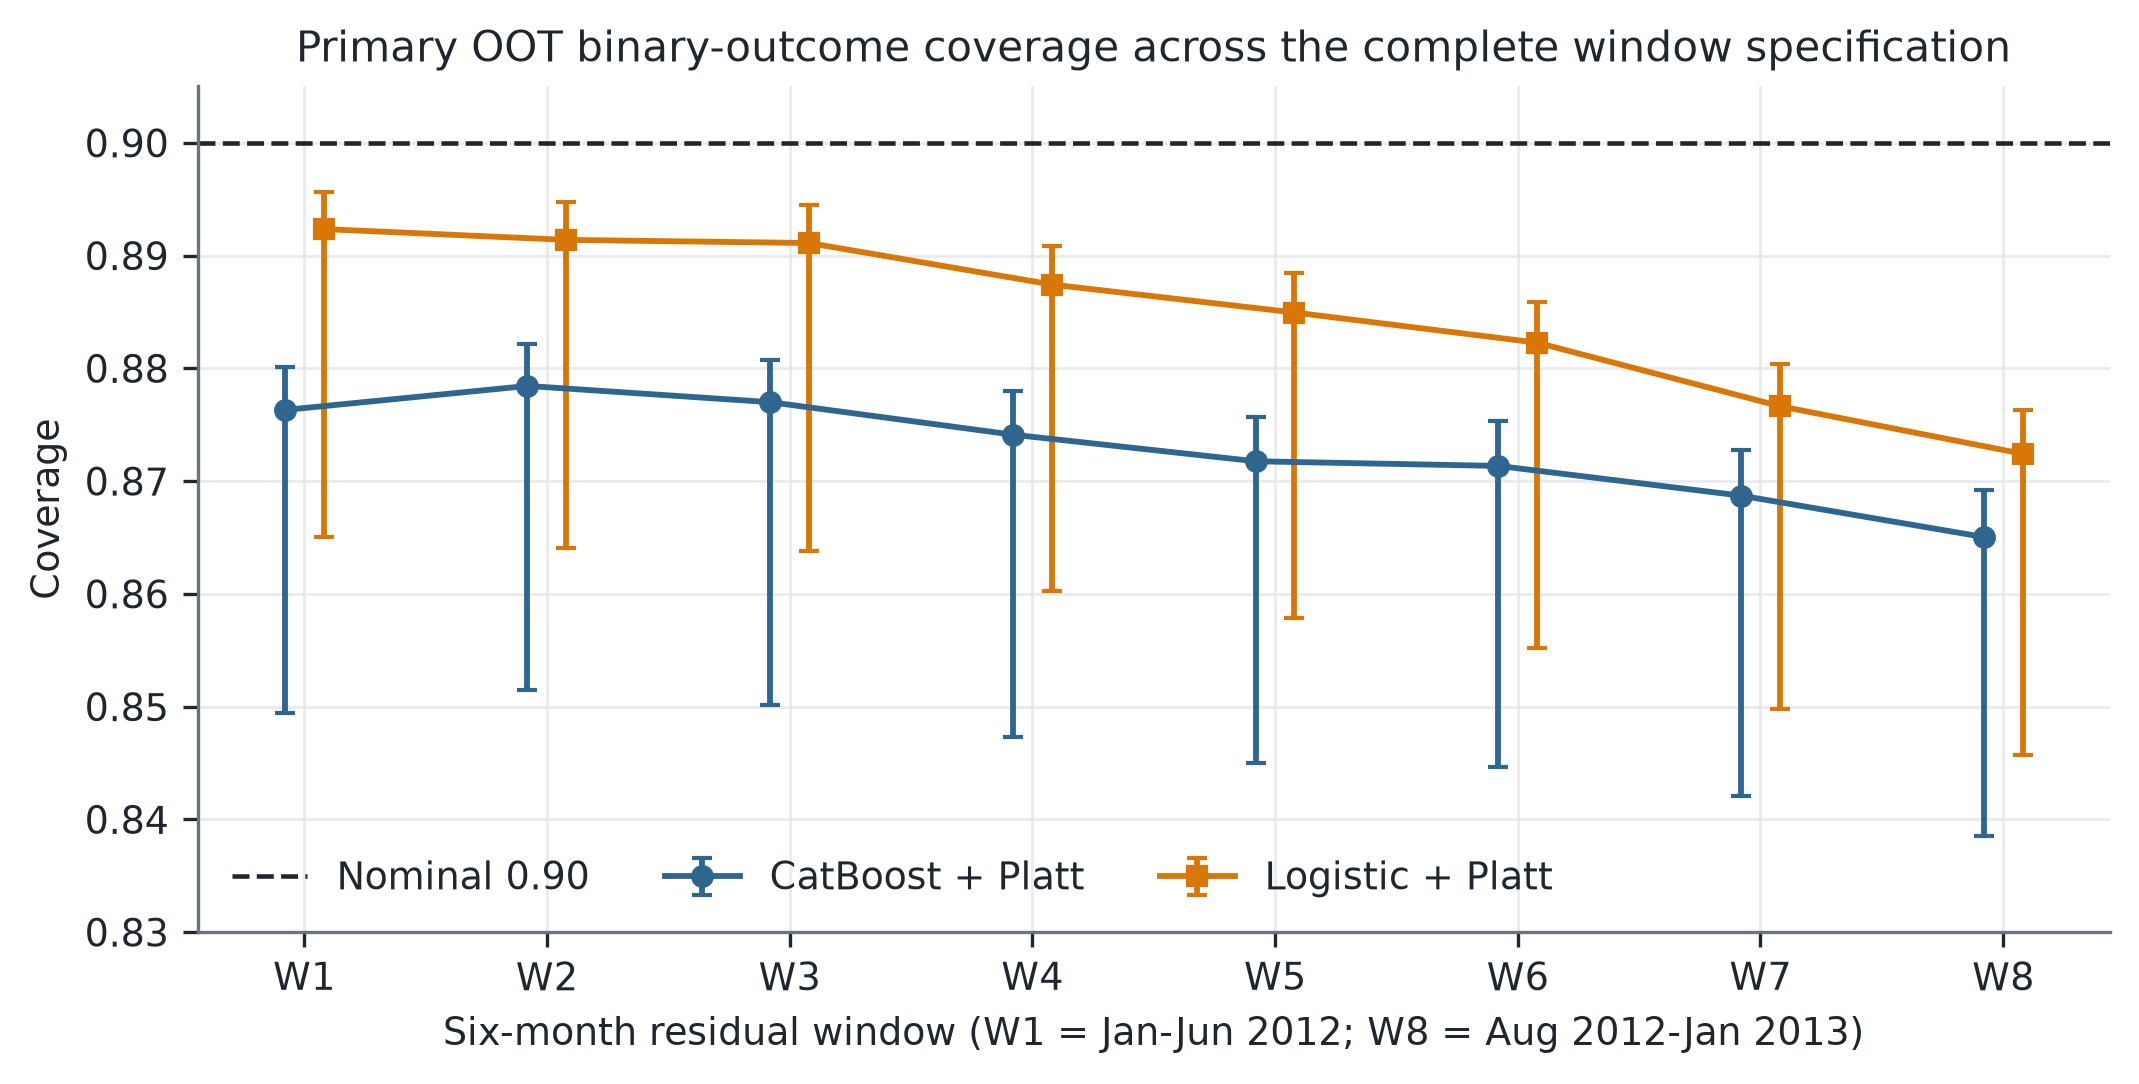
\includegraphics[width=0.95\linewidth,height=\textheight,keepaspectratio]{../../reports/crpto/figures/crpto_ijds_v4_fig1_coverage.png}

}

\caption{\label{fig-coverage}Resolved coverage and sharp completion
bounds appear in Panel A. Panel B marks cells meeting the locked nominal
reporting thresholds for the stronger joint-block reference. Segments
are identification bounds, not error bars; flags have no post-selection
FWER interpretation.}

\end{figure}%

Supplement Tables S6--S6A report every bound and set-geometry component.

The closed 1-, 2-, 5-, and 10-stratum grid leaves all 64 CatBoost and
numeric-logistic primary-window upper bounds below 0.90 (maximum
0.897294), so the five-stratum taxonomy is not selected as a favorable
exception. A deliberately more censored 2017 extension is mixed:
CatBoost remains below nominal in 8/8 windows (maximum 0.895157),
whereas numeric logistic is below in 2/8 and its other six sharp
intervals contain 0.90 (maximum 0.908928). The extension is a stress
with 28,936 unresolved outcomes, not primary OOT evidence, an
independent replication, or a transport repair.

Across all 40 cells, coverage among administratively resolved
nondefaults is 0.982982--0.992714 versus 0.232570--0.363916 among
resolved defaults. This conditions on resolution and observed label, so
it is not all-candidate label-conditional validity, equalized coverage,
or a fairness test.

Set efficiency supplies a different view over all 376,890 candidates.
Across the same 40 cells, AvgC is 1.128128--1.268134, empty sets account
for 0.67\%--1.61\%, two-label sets for 14.42\%--27.48\%, and singletons
for 71.85\%--83.97\%. These components show that mean cardinality alone
would hide both never-covered and uninformative cases; none is a
validity guarantee. We summarize discrimination by the area under the
receiver operating characteristic curve (AUC).

\begin{longtable}[]{@{}lrrrr@{}}
\caption{Five-model coverage audit; predictive metrics use 364,814
resolved outcomes and coverage retains all 376,890
candidates.}\label{tbl-credit-controls}\tabularnewline
\toprule\noalign{}
Score & OOT AUC & Brier & Slope & \(U_{\max}\) \\
\midrule\noalign{}
\endfirsthead
\toprule\noalign{}
Score & OOT AUC & Brier & Slope & \(U_{\max}\) \\
\midrule\noalign{}
\endhead
\bottomrule\noalign{}
\endlastfoot
CatBoost & 0.6406 & 0.1299 & 0.7954 & 0.8826 \\
Logistic & 0.6420 & 0.1288 & 0.5432 & 0.8962 \\
Monotone CB & 0.6520 & 0.1286 & 0.8351 & 0.8865 \\
Platform WOE & 0.6331 & 0.1295 & 0.9187 & 0.8949 \\
Pricing-excluded WOE & 0.6129 & 0.1302 & 0.7098 & 0.8977 \\
\end{longtable}

Among administratively resolved candidates, all five mean calibration
errors are negative and all calibration slopes are below one. AUC,
Brier, and calibration summaries condition on resolution; WOE/IV and PSI
are descriptive for separate design reasons and are not validity tests,
a model contest, or an identified explanation of the coverage gap.

\subsubsection{Secondary post-inspection joint-block
reference}\label{secondary-post-inspection-joint-block-reference}

A secondary combined-rank diagnostic has 31 of 40 cell-level reference
tail areas meeting the locked nominal reporting thresholds. Its null is
stronger than the condition split conformal needs and its family was
inspected before the lock, so it carries no post-selection FWER or
theorem-failure interpretation and nonflags establish no
exchangeability. Online Supplement B.4.1 reports it in full.

The retrospective Label-Mondrian sensitivity
\citep{vovk2012conditional, ding2023} raises observed default coverage
in the resolved panel, yet still leaves 27/40 marginal and 109 of 400
label-stratum bounds below nominal. Relative to the baseline ranges
above, AvgC rises to 1.724--1.785 and two-label sets to
72.37\%--78.55\%; all 40 aggregate class-gap bounds cross zero. It
therefore neither uniformly repairs coverage nor establishes
within-label exchangeability.

All 24 encoding cells remain below 0.90 across sentinel, indicator, and
native-null variants (maxima 0.8826, 0.8843, 0.8800). The 16
individual-age cells at 39-calendar-month cutoffs for the 2016 and 2017
origins also remain below (maxima 0.8791 and 0.8753), as do all 32 cells
from four declared completions of 215 cutoff-unavailable fit labels.
These shared-chronology sensitivities are neither independent
replications nor exact day-age matches.

\subsection{Closed calibrator-family sensitivity does not establish a
uniform
shortfall}\label{closed-calibrator-family-sensitivity-does-not-establish-a-uniform-shortfall}

The separate CatBoost calibrator audit holds the base-score panel,
common five-stratum taxonomy, eight residual windows, six-month
outcome-availability rule, and loan-wise unresolved-outcome treatment
fixed. It reports all four frozen maps without using OOT results to
select among them:

\begin{longtable}[]{@{}
  >{\raggedright\arraybackslash}p{(\linewidth - 10\tabcolsep) * \real{0.1304}}
  >{\raggedleft\arraybackslash}p{(\linewidth - 10\tabcolsep) * \real{0.1739}}
  >{\raggedleft\arraybackslash}p{(\linewidth - 10\tabcolsep) * \real{0.1739}}
  >{\raggedleft\arraybackslash}p{(\linewidth - 10\tabcolsep) * \real{0.1739}}
  >{\raggedleft\arraybackslash}p{(\linewidth - 10\tabcolsep) * \real{0.1739}}
  >{\raggedleft\arraybackslash}p{(\linewidth - 10\tabcolsep) * \real{0.1739}}@{}}
\caption{Closed four-map CatBoost sensitivity. Bounds are sharp
identification intervals for this archive, not confidence intervals.
}\label{tbl-calibrator-sensitivity}\tabularnewline
\toprule\noalign{}
\begin{minipage}[b]{\linewidth}\raggedright
CatBoost score map
\end{minipage} & \begin{minipage}[b]{\linewidth}\raggedleft
Overall upper \(<.90\)
\end{minipage} & \begin{minipage}[b]{\linewidth}\raggedleft
Lowest lower
\end{minipage} & \begin{minipage}[b]{\linewidth}\raggedleft
Highest upper
\end{minipage} & \begin{minipage}[b]{\linewidth}\raggedleft
Resolved-coverage range
\end{minipage} & \begin{minipage}[b]{\linewidth}\raggedleft
AvgC range
\end{minipage} \\
\midrule\noalign{}
\endfirsthead
\toprule\noalign{}
\begin{minipage}[b]{\linewidth}\raggedright
CatBoost score map
\end{minipage} & \begin{minipage}[b]{\linewidth}\raggedleft
Overall upper \(<.90\)
\end{minipage} & \begin{minipage}[b]{\linewidth}\raggedleft
Lowest lower
\end{minipage} & \begin{minipage}[b]{\linewidth}\raggedleft
Highest upper
\end{minipage} & \begin{minipage}[b]{\linewidth}\raggedleft
Resolved-coverage range
\end{minipage} & \begin{minipage}[b]{\linewidth}\raggedleft
AvgC range
\end{minipage} \\
\midrule\noalign{}
\endhead
\bottomrule\noalign{}
\endlastfoot
Platt & 8/8 & 0.842485 & 0.882597 & 0.865855--0.879166 &
1.128128--1.183942 \\
Isotonic & 1/8 & 0.870307 & 0.927345 & 0.892786--0.924940 &
1.199517--1.385794 \\
Beta (\texttt{abm}) & 8/8 & 0.842485 & 0.882597 & 0.865855--0.879166 &
1.128128--1.183942 \\
IVAP Venn--Abers scalar & 1/8 & 0.869933 & 0.922609 & 0.892455--0.920047
& 1.198090--1.359553 \\
\end{longtable}

Only 18 of the 32 overall upper bounds are below 0.90. Across the eight
pooled shared-completion contrasts, every isotonic-minus-Platt
finite-archive coverage-difference bound is strictly positive (all bound
endpoints across windows, 0.026069--0.055019), as is every
IVAP-minus-Platt bound (0.025748--0.049587); Platt-minus-beta is exactly
\([0,0]\) in all 48 pooled-plus-stratum cells. These paired bounds
describe the finite archive; they do not rank calibrators. For both
isotonic and Venn--Abers, W2--W4 have lower bounds above 0.90, W1 and
W5--W7 contain 0.90, and only W8 lies below it. Platt and beta yield
identical aggregate set-geometry counts and coverage estimates and
bounds in all 48 pooled-plus-stratum cells, although their scalar scores
and continuous interval widths are not identical. The active Platt
branch reconciles all 48 corresponding baseline rows to maximum absolute
difference \(2.22\times10^{-16}\).

The registered Table S6O rows also expose the atoms created by the
piecewise-constant isotonic and IVAP maps. W2--W4 share one
aggregate-bound row, while W1 and W5--W7 share another. W8 has the
latter overall residual-quantile summary but different aggregate bounds
after the frozen five-stratum construction. This is the empirical atomic
case anticipated by Lemma 1, and it shows why equality of one pooled
threshold summary is insufficient to determine the full stratified set
construction.

The supported interpretation is therefore that a family-wide shortfall
is not established: the Platt result is not a uniform property of this
closed score-map family. This evidence leaves true-coverage dependence
unestablished, selects no preferable map, and cannot transfer the Venn
multiprobability guarantee to its scalarization. Supplement Table S2C
reports the four same-sample fit diagnostics; machine-readable Tables
S6O and S6P report all 192 method--window--scope cells and all 288
shared-completion pairwise cells. This sensitivity performs no portfolio
optimization: the separate primary analysis continues to use the
pre-existing Platt score, and none of the three alternative maps is
propagated.

\subsection{Marginal score and residual-distribution
transport}\label{marginal-score-and-residual-distribution-transport}

The complete five-learner target panel identifies outcome prevalence as
{[}0.151163, 0.183205{]} under unrestricted completion of the 12,076
unresolved binary outcomes. Mean scores range from 0.108968 to 0.127230.
Consequently, every sharp interval for mean score minus outcome
prevalence is below zero: the five upper bounds range from -0.042196 to
-0.023934. The common identification width, 0.032041, is exactly the
unresolved fraction. This is a finite-panel marginal level gap. Read
with the registered calibration and target prevalence summaries, it is
consistent with an increase in class prevalence, which is the marginal
signature associated with label shift. It cannot identify label shift,
establish invariance of \(P(X\mid Y)\), separate label from covariate
shift, estimate individual or class-conditional calibration, rank
learners, or infer a cause of the coverage shortfall.

Online Supplement D.5.1 proves the pointwise target-CDF sandwich
obtained by assigning every unresolved residual its attainable minimum
or maximum; monotonicity of the two one-sided suprema then gives the
four cellwise sharp extrema. The residual-distribution audit evaluates
both discrepancies in all 200 learner--window--stratum cells. In 158
cells, the entire calibration-minus-target discrepancy range lies above
the reverse range; in 8, the reverse range lies above; and in 34 the two
are not robustly ordered. The corresponding 3,000-cell monthly census is
2,140, 488, and 372. These labels compare the magnitudes of two
directional suprema: they are neither stochastic-dominance statements
nor Kolmogorov--Smirnov (KS) tests, identify no transport mechanism, and
cellwise sharpness cannot make the bound endpoints jointly attainable
across cells. Online Supplement Tables S6L--S6N report the learner
census, all pooled cells, and the marginal gaps.

\subsection{Complete calibration-side binary phase
census}\label{complete-calibration-side-binary-phase-census}

A clean calibration-only replay evaluates Proposition 1 over the
complete frozen design: five learners, eight windows, and five ordered
score strata, or 200 cells. It uses calibration labels to form residuals
but reads no target panel or evaluation outcome, optimization output, or
funded allocation. Both calibration classes are nonempty and the
finite-sample rank is uncapped in all 200 cells. Recomputed thresholds,
residual tie counts, score extrema, rank brackets, and the frozen
threshold agree in every cell; the maximum absolute threshold gap is
zero.

\begin{longtable}[]{@{}
  >{\raggedleft\arraybackslash}p{(\linewidth - 10\tabcolsep) * \real{0.1667}}
  >{\raggedleft\arraybackslash}p{(\linewidth - 10\tabcolsep) * \real{0.1667}}
  >{\raggedleft\arraybackslash}p{(\linewidth - 10\tabcolsep) * \real{0.1667}}
  >{\raggedleft\arraybackslash}p{(\linewidth - 10\tabcolsep) * \real{0.1667}}
  >{\raggedleft\arraybackslash}p{(\linewidth - 10\tabcolsep) * \real{0.1667}}
  >{\raggedleft\arraybackslash}p{(\linewidth - 10\tabcolsep) * \real{0.1667}}@{}}
\caption{Complete calibration-side phase census with no
target/evaluation outcomes. Reader-facing stratum \(s\) equals internal
zero-based \protect\texttt{conformal\_group} plus one. Applicability
columns name sufficient conditions under which the corresponding
phase-margin checks are invoked; they are not failures in the remaining
cells. }\label{tbl-phase-census}\tabularnewline
\toprule\noalign{}
\begin{minipage}[b]{\linewidth}\raggedleft
Ordered score stratum
\end{minipage} & \begin{minipage}[b]{\linewidth}\raggedleft
Cells
\end{minipage} & \begin{minipage}[b]{\linewidth}\raggedleft
\(c<1/2\)
\end{minipage} & \begin{minipage}[b]{\linewidth}\raggedleft
\(m\le0\)
\end{minipage} & \begin{minipage}[b]{\linewidth}\raggedleft
\(\max p<1/2\) applicable
\end{minipage} & \begin{minipage}[b]{\linewidth}\raggedleft
No-interleaving applicable
\end{minipage} \\
\midrule\noalign{}
\endfirsthead
\toprule\noalign{}
\begin{minipage}[b]{\linewidth}\raggedleft
Ordered score stratum
\end{minipage} & \begin{minipage}[b]{\linewidth}\raggedleft
Cells
\end{minipage} & \begin{minipage}[b]{\linewidth}\raggedleft
\(c<1/2\)
\end{minipage} & \begin{minipage}[b]{\linewidth}\raggedleft
\(m\le0\)
\end{minipage} & \begin{minipage}[b]{\linewidth}\raggedleft
\(\max p<1/2\) applicable
\end{minipage} & \begin{minipage}[b]{\linewidth}\raggedleft
No-interleaving applicable
\end{minipage} \\
\midrule\noalign{}
\endhead
\bottomrule\noalign{}
\endlastfoot
1 & 40 & 40 & 40 & 40 & 40 \\
2 & 40 & 40 & 40 & 40 & 40 \\
3 & 40 & 7 & 7 & 40 & 40 \\
4 & 40 & 0 & 0 & 40 & 40 \\
5 & 40 & 0 & 0 & 24 & 28 \\
\textbf{Total} & \textbf{200} & \textbf{87} & \textbf{87} & \textbf{184}
& \textbf{188} \\
\end{longtable}

The exact general count criterion \(c<1/2\iff A+B\ge k\) passes in all
200 cells. The simpler equivalence \(c<1/2\iff m\le0\) passes in all 184
cells where every calibration score is below one half. The stated
threshold-source branch passes in all 188 cells satisfying no
interleaving. Therefore the archived 40/40/7/0/0 pattern is complete for
this frozen grid, not a selected low-stratum anecdote. It remains
retrospective and calibration-side. The census supports no universal
phase law, target-side inference, or decision guarantee. Online
Supplement Table S6I reports all 200 cells.

\subsection{Fixed-panel response and an illustrative phase-margin
crossing}\label{fixed-panel-response-and-an-illustrative-phase-margin-crossing}

The common-panel replay reports all 175 learner--stratum--transition
contrasts and 35 learner-level aggregates. Resolved-panel responses
range from -1.22645 to +1.01550 percentage points. Sharp all-candidate
identification widths have median 0.0185, 90th percentile 0.1063, and
maximum 0.2346 percentage points. Among the 175 stratum rows, 122 sharp
intervals are strictly negative, 48 are strictly positive, and five
equal \([0,0]\); those signs mechanically follow threshold direction,
whereas the crossed mass, response magnitude, and identification width
quantify the finite target response.

Against that complete census, CatBoost S3 supplies an illustration
selected after inspection solely for that purpose. It is the third score
stratum (internal zero-based group 2), which the published tables encode
as \texttt{score\_stratum} 3. Fit prevalence declines from 0.1167 in W1
to 0.1017 in W7, then to 0.0971 in W8. The nominal \(\alpha=0.10\)
crossing is only shorthand: the exact finite coordinate changes from
\(m=+11\) with \((n-k)/n=592/5{,}929=0.099848\) to \(m=-16\) with
\(622/6{,}238=0.099711\). Because both calibration blocks lie below one
half, W7's threshold is one minus the 11th largest default score,
whereas W8's is the 5,616th smallest of 5,632 nondefault scores; these
are distinct overlapping blocks, not a unitary flip between two class
maxima. The fitted residual quantile falls from 0.8884 to 0.1118; mean
OOT width in the stratum falls from 0.9843 to 0.2076. Its discrete
intersection simultaneously moves from 0.96\% \(\{0,1\}\) and 99.04\%
\(\{0\}\) in W7 to 0\% \(\{0,1\}\), 99.74\% \(\{0\}\), and 0.26\% empty
in W8. This stratum and transition were selected after inspection solely
as a descriptive geometric illustration; they are not confirmatory and
select no learner, stratum, or window. All 175 adjacent contrasts remain
reported.

\begin{figure}

\centering{

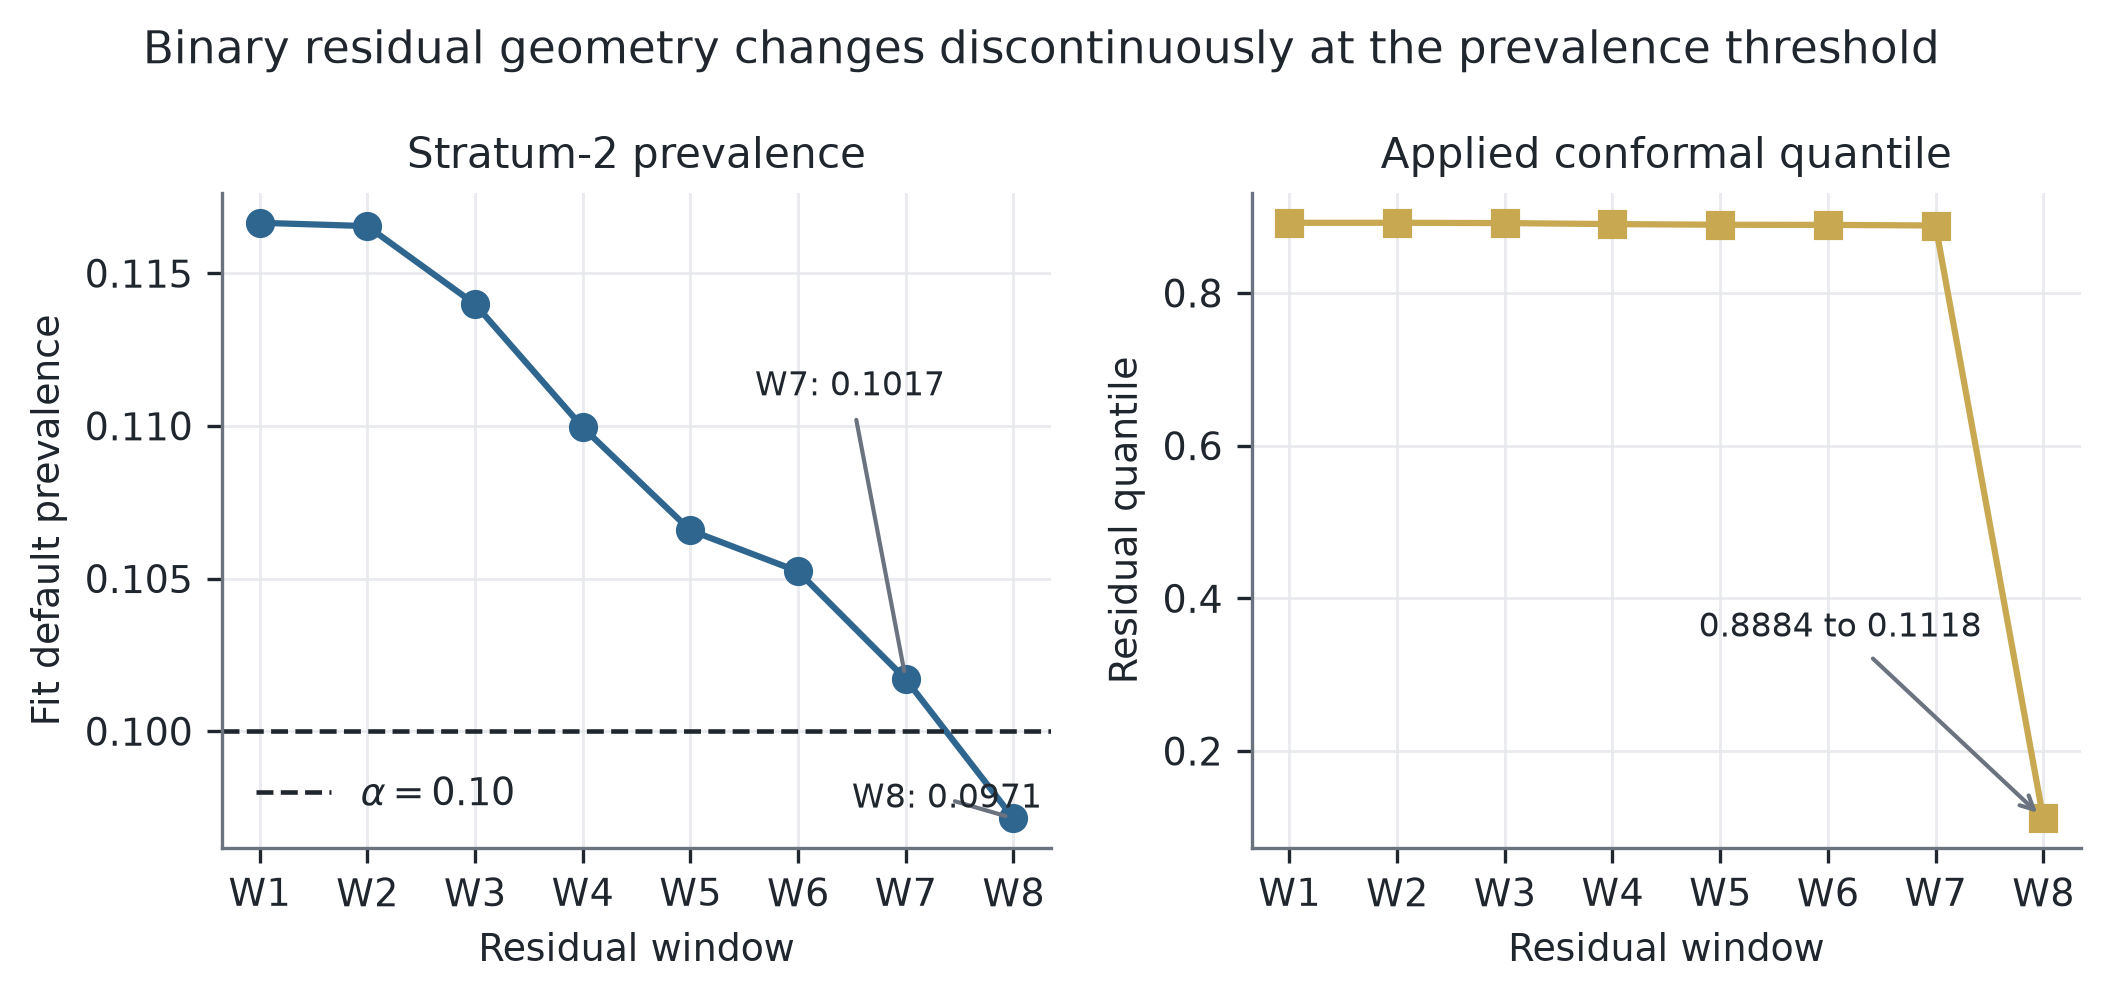
\includegraphics[width=0.82\linewidth,height=\textheight,keepaspectratio]{../../reports/crpto/figures/crpto_ijds_v4_fig2_phase_transition.png}

}

\caption{\label{fig-phase}Post-inspection illustration: CatBoost S3 fit
prevalence, finite-sample boundary, and fitted residual threshold across
eight overlapping windows, shown on focused scales. The illustrated pair
changes from phase margin +11 in W7 to -16 in W8 and coincides with the
large threshold step described by Proposition 1's conditional
order-statistic characterization; it is not confirmatory or a winner,
and all 175 contrasts remain reported.}

\end{figure}%

The common-panel replay evaluates the target response directly. In the
highlighted S3, the same 79,047 loans appear under both thresholds.
Among 76,495 resolved loans, 164 nondefaults and 117 defaults cross out
of coverage, so the exact response is \(-281/76{,}495=-0.003673\).
Optimizing over assignments that give each of the 2,552 unresolved loans
the same label under both thresholds, the all-candidate response is
sharply \([-312,-290]/79{,}047=[-0.003947,-0.003669]\). Thus the large
threshold step and the much smaller realized coverage response are
compatible because only target mass in the crossed bands matters. In the
unresolved subset, 9 loans lie in both signed bands and leave coverage
under either label, while 22 lie in exactly one and generate the
identification width.

At stratum level, fixed-target coverage is monotone in \(c\), so the
response sign is mechanically determined by the threshold direction; its
census is an implementation-consistency check, not a discovery. No
stratum interval strictly straddles or one-sidedly touches zero. At
learner level the five stratum thresholds can move in different
directions; after summing their integer numerators before division, all
35 transition intervals exclude zero: 31 are negative and 4 positive.
These are deterministic finite-archive descriptions after optimizing
over loan-level labels shared within each contrast. Their role is
descriptive: no hypothesis test, temporal-validity guarantee,
independent replication, or ranking is claimed. Sharpness is cellwise:
the manuscript makes no claim that every bound endpoint across all 175
overlapping contrasts is jointly attained by one global completion.
Figure~\ref{fig-common-panel} therefore places the resolved and
all-candidate quantities in separate aligned panels: they share axes but
not denominators, and the all-candidate segments are identification
bounds rather than uncertainty intervals around the resolved response.

\begin{figure}

\centering{

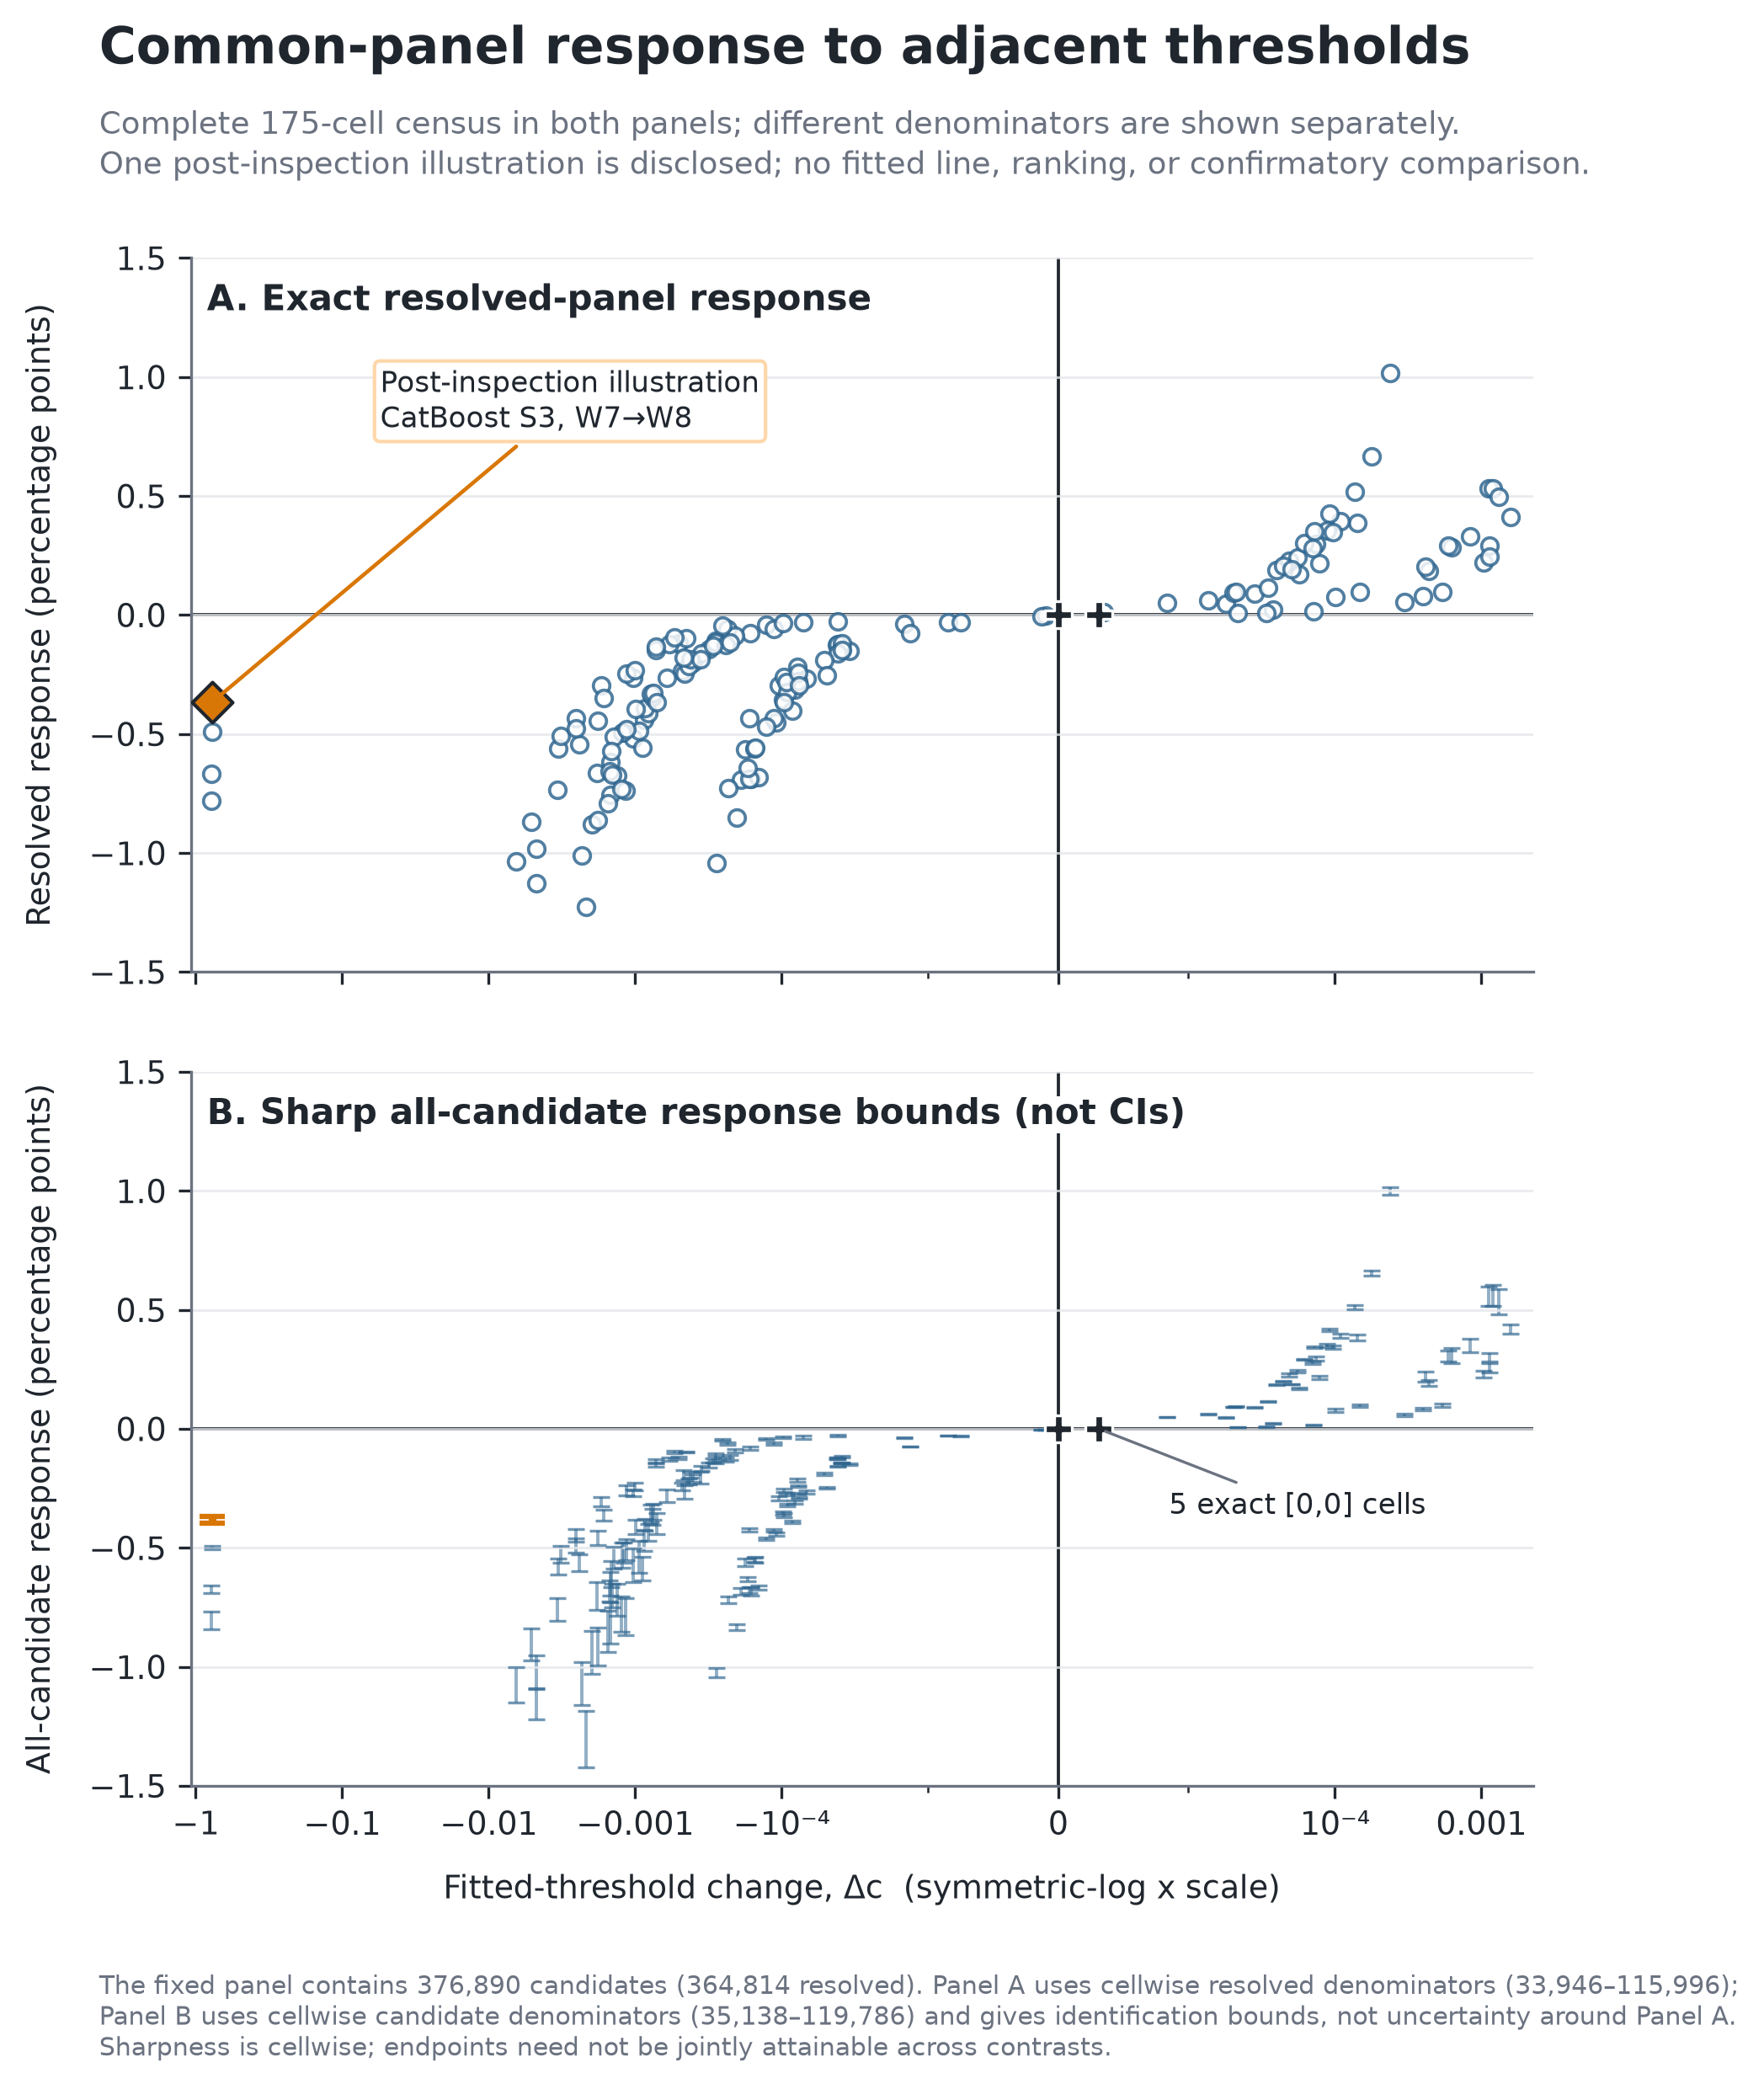
\includegraphics[width=0.92\linewidth,height=\textheight,keepaspectratio]{../../reports/crpto/figures/crpto_ijds_v4_fig4_common_panel_threshold_response.png}

}

\caption{\label{fig-common-panel}Fixed-panel response for all 175
learner--stratum--transition cells. Panel A gives resolved-panel
changes; Panel B gives sharp all-candidate bounds with each unresolved
loan's label held fixed under both thresholds. The aligned panels have
different denominators. Capped segments are identification bounds,
orange marks the post-inspection S3 illustration, and black crosses mark
the five \([0,0]\) cells; no regression, ranking, confirmatory,
continuity, or joint-attainability claim is made.}

\end{figure}%

Proposition 1 gives the exact conditional order-statistic
characterization of each frozen block, but score binning itself cannot
guarantee ordered finite-bin prevalences, a crossing of \(\alpha\), or
any low-regime stratum. A phase-margin statement is calibration-side;
zero positive-class target coverage additionally requires the stated
target condition. W7 and W8 are overlapping but distinct calibration
blocks, so their thresholds cannot be represented as the two sides of
one fixed block with a shared pair of class maxima. The narrower W8
interval still leaves S3 coverage at {[}0.8225, 0.8547{]}. The
common-panel response calculation shows what changed on the frozen
target set, but it cannot identify why the calibration threshold moved
or why the target mass occupies those bands. In W8, \(1-c=0.888199\)
exceeds the maximum target S3 score 0.111893, so no positive label can
be covered; this conditional support fact still supplies neither a
transport guarantee nor a cause. Online Supplement B.5.1 gives the full
integer identities and tables.

Fit-label lags 0, 3, and 6 months retain more than 99\% in every month
and preserve the crossing; 8 and 12 months retain only 98.68\% and
97.45\% in their weakest month and fail the rule. This is stability
within the retained lag family, not a causal claim.

Observed-only, all-nondefault, and later-terminal completion retain the
W7--W8 crossing. All-default completion instead gives prevalences
0.105974/0.100287 and quantiles near 0.889, removing the crossing while
all eight overall upper bounds remain below 0.90. Nonlinear refits make
these four scenarios declared stresses, not sharp bounds over
\(2^{215}\) assignments; the observed phase path is not
scenario-invariant.

Fit-label timing refits recipes; evaluation-outcome availability instead
holds scores, supports, and allocations fixed. The axes were not
crossed, so they do not establish joint lag robustness.

\subsection{Set-preserving embedding sensitivity: allocation change and
direction
noninvariance}\label{set-preserving-embedding-sensitivity-allocation-change-and-direction-noninvariance}

The set-preserving sensitivity varies \(\theta\in\{0,.25,.50,.75,1\}\)
in Equation~\ref{eq-set-preserving-embedding} jointly with the five
declared \(\gamma\) values, both outcome-blind rulers, all three
coordinates, eight windows, and fifteen primary months. Every one of the
80 role--window--\(\theta\) diagnostics preserves every binary set
exactly, even though the largest contraction of a continuous upper bound
endpoint is 0.892012. Among the 11,520 outcome-free monthly contrasts
with \(\theta>0\) and \(\gamma>0\), the normalized exposure vector
changes by more than \(10^{-10}\) in 9,659 (83.85\%): 5,760/5,760 under
the normalized-score ruler and 3,899/5,760 under objective matching.
When \(\gamma=0\), the embedding drops out of the score as it should.
All 2,880 outcome-free monthly controls have zero exposure distance and
objective difference; the 2,880 monthly and 192 pooled evaluation
controls have zero objective and outcome contrasts.

The outcome evaluation freezes those allocations before joining the
outcome panel and compares each \(\theta>0\) portfolio with its
\(\theta=0\) counterpart using one loan-wise completion on the funded
union. Across the 768 pooled noncontrol contrasts for each metric, the
complete direction census is:

\begin{longtable}[]{@{}
  >{\raggedright\arraybackslash}p{(\linewidth - 8\tabcolsep) * \real{0.1579}}
  >{\raggedleft\arraybackslash}p{(\linewidth - 8\tabcolsep) * \real{0.2105}}
  >{\raggedleft\arraybackslash}p{(\linewidth - 8\tabcolsep) * \real{0.2105}}
  >{\raggedleft\arraybackslash}p{(\linewidth - 8\tabcolsep) * \real{0.2105}}
  >{\raggedleft\arraybackslash}p{(\linewidth - 8\tabcolsep) * \real{0.2105}}@{}}
\caption{Pooled set-preserving-embedding direction census after
excluding the \(\gamma=0\) controls. \emph{Not separated} means that the
sharp interval contains zero beyond the metric tolerance; \emph{within
tolerance} means both interval bounds are within that tolerance. Signs
are numerical, not uniformly favorable or
adverse.}\label{tbl-embedding-direction}\tabularnewline
\toprule\noalign{}
\begin{minipage}[b]{\linewidth}\raggedright
Metric, \(\theta>0\) minus \(\theta=0\)
\end{minipage} & \begin{minipage}[b]{\linewidth}\raggedleft
Negative
\end{minipage} & \begin{minipage}[b]{\linewidth}\raggedleft
Positive
\end{minipage} & \begin{minipage}[b]{\linewidth}\raggedleft
Not separated
\end{minipage} & \begin{minipage}[b]{\linewidth}\raggedleft
Within tolerance
\end{minipage} \\
\midrule\noalign{}
\endfirsthead
\toprule\noalign{}
\begin{minipage}[b]{\linewidth}\raggedright
Metric, \(\theta>0\) minus \(\theta=0\)
\end{minipage} & \begin{minipage}[b]{\linewidth}\raggedleft
Negative
\end{minipage} & \begin{minipage}[b]{\linewidth}\raggedleft
Positive
\end{minipage} & \begin{minipage}[b]{\linewidth}\raggedleft
Not separated
\end{minipage} & \begin{minipage}[b]{\linewidth}\raggedleft
Within tolerance
\end{minipage} \\
\midrule\noalign{}
\endhead
\bottomrule\noalign{}
\endlastfoot
Standardized payoff & 128 & 338 & 230 & 72 \\
Funded default & 350 & 157 & 173 & 88 \\
Funded binary miscoverage & 340 & 259 & 81 & 88 \\
\end{longtable}

Across 576 four-\(\theta\) tracks, direction changes within 324 and 77
contain both tolerance-separated signs (96 under the zero-tolerance
geometric sign). Equal binary sets therefore do not identify invariant
allocations or descriptive outcome directions over this grid. This
locked post-inspection sensitivity selects no audited dimension. It
supplies no set-native or validity repair; outcome direction remains
retrospective and cellwise. Online Supplement Tables S9K--S9L report the
outcome-free allocation census and both contrast families.

\subsubsection{Global score-equivalence
certificate}\label{global-score-equivalence-certificate}

Because Proposition 2 concerns every allocation in a menu, the replay
certifies the full-budget affine hull of all 26 role--month menus
(dimension \(n-1\); 6,011--28,106 candidates) before evaluating every
declared score pair. The global certificate holds on the 1,872 identity
controls (\(\theta=0\), or \(\theta>0\) with \(\gamma=0\)) and fails on
all 3,328 informative \(\theta,\gamma>0\) comparisons and all 6,240
closed-calibrator pairs. Failure withholds global order equivalence; it
cannot force an allocation change at a fixed cell or unequal optimal
faces, and the calibrator rows also change the payoff coefficient. This
outcome-free, no-optimization reconciliation appears in Online
Supplement Table S9M.

\subsection{Set-native binary worst-label counterpart with declared
empty-set
fail-closure}\label{set-native-binary-worst-label-counterpart-with-declared-empty-set-fail-closure}

The compatible continuous fibre in
Equation~\ref{eq-compatible-embedding-fibre} has no informative
rectangular worst-case loan ordering. A different, explicitly set-native
risk coefficient is nevertheless available if the protected object is
the binary label set itself. Define

\begin{equation}\protect\phantomsection\label{eq-set-native-worst-label}{
r_i(S_i)=
\begin{cases}
0,&S_i=\{0\},\\
1,&S_i\in\{\varnothing,\{1\},\{0,1\}\}.
\end{cases}
}\end{equation}

For nonempty sets this is the worst admissible binary label; the
empty-set value one is a declared fail-closed decision convention, not a
conformal theorem. The score is invariant to every continuous embedding
of the same binary set. Only this risk coefficient is set-native: the
plug-in payoff objective and other optimization components retain
\(p_i\). Moreover, marginal coverage cannot endow the Cartesian product
with a joint-coverage guarantee, and the temporal archive lacks the
exchangeability needed for a probabilistic robust guarantee.

The outcome-free phase reports all 1,248
window--role-month--ruler--coordinate frontier cells, including all 720
primary cells, 126,686 positive funded rows, 208 taxonomy rows, and
1,248 solver-audit rows. Every portfolio exhausts the budget. Same-order
replay is exact; reversed-order differences are at most
\(1.75\times10^{-10}\) in the objective and \(3.01\times10^{-14}\) in
normalized exposure, and the independent-solver objective-rate
discrepancy is at most \(2.04\times10^{-16}\).

After those allocations are frozen, Phase B compares each worst-label
primary cell with all 25 continuous-embedding \(\theta\)--\(\gamma\)
cells at the same window, month, ruler, and coordinate, using one
loan-wise binary completion on each funded union. The complete
worst-label-minus-continuous-embedding pooled census is:

\begin{longtable}[]{@{}lrrrr@{}}
\caption{Pooled set-native-worst-label-minus-continuous-embedding
direction partition. Positive payoff is favorable; positive default or
miscoverage is adverse. Each cell is sharp separately under a shared
completion, while bound endpoints across overlapping cells are not
asserted jointly
attainable.}\label{tbl-set-native-direction}\tabularnewline
\toprule\noalign{}
Metric & Positive & Negative & Contains zero & Total \\
\midrule\noalign{}
\endfirsthead
\toprule\noalign{}
Metric & Positive & Negative & Contains zero & Total \\
\midrule\noalign{}
\endhead
\bottomrule\noalign{}
\endlastfoot
Standardized payoff & 15 & 1,065 & 120 & 1,200 \\
Funded default & 1,196 & 0 & 4 & 1,200 \\
Funded binary miscoverage & 1,009 & 120 & 71 & 1,200 \\
\end{longtable}

Thus removing the unidentified continuous embedding establishes no
transport or validity repair and no uniform outcome dominance in this
archive: the default contrast is adverse in 1,196/1,200 pooled cells and
never favorable, while payoff is lower in 1,065. The observed
coexistence is consistent with the coarse score assigning zero to the
very large singleton-nondefault class and leaving the plug-in payoff
objective and remaining constraints to determine choices within
risk-score ties; it is not a causal mechanism. The grid selects no
operating object and carries no inferential or prospective validity.
Online Supplement Table S9N reports all 75 \(\theta\)--\(\gamma\) by
metric partitions at monthly and pooled levels.

\subsubsection{Fully set-native structural
boundary}\label{fully-set-native-structural-boundary}

If the payoff coefficient is also the set-internal minimum, Supplemental
Remark D.2.2 shows that every loan outside the singleton-\(\{0\}\) class
has payoff \(-\mathrm{LGD}\) and constructed set risk one. Under exact
budget, no cash, bounded loan exposures, an exhaustive disjoint
upper-purpose-cap partition, nonnegative rates, positive LGD,
fail-closed empty-set completion, and feasible full-budget
singleton-zero support, substitution therefore confines every maximin
optimizer to singleton-zero loans and makes the complete optimal face
and value invariant over caps in \([0,1]\). The feasibility premise
passes in all 208 window-by-role-month certificates over 26 candidate
menus using the primary CatBoost--Platt specification (88 development
and 120 target certificates), reconciled from hash-pinned predecessor
solves with zero new optimization (Online Supplement Table S9O). This is
a conditional structural stop rule, not evidence of true zero risk,
joint or selected-set validity, optimizer uniqueness, outcome dominance,
or a deployable policy.

\subsection{Path-end contrast direction changes with ruler and
coordinate}\label{path-end-contrast-direction-changes-with-ruler-and-coordinate}

The two-ruler freeze contains 6,240 portfolios, and the evaluator
reports all 720 monthly and 48 complete-window path-end contrasts.
Table~\ref{tbl-two-ruler} reports \(\gamma=1\) minus \(\gamma=0\);
\emph{adverse} means lower payoff and higher default/miscoverage, while
\emph{crossing} means the sharp interval contains zero. Each row is one
ruler-coordinate track over the same fifteen OOT menus. The eight
windows are overlapping residual specifications, so the table is a
six-track census, not independent replications or votes.

\begin{longtable}[]{@{}
  >{\raggedright\arraybackslash}p{(\linewidth - 6\tabcolsep) * \real{0.2000}}
  >{\raggedleft\arraybackslash}p{(\linewidth - 6\tabcolsep) * \real{0.2667}}
  >{\raggedleft\arraybackslash}p{(\linewidth - 6\tabcolsep) * \real{0.2667}}
  >{\raggedleft\arraybackslash}p{(\linewidth - 6\tabcolsep) * \real{0.2667}}@{}}
\caption{Six protocol-locked path-end tracks, reported as the envelope
over the eight overlapping residual windows. Full window-specific sharp
bounds are in Online Supplement Table
S9.}\label{tbl-two-ruler}\tabularnewline
\toprule\noalign{}
\begin{minipage}[b]{\linewidth}\raggedright
Ruler / coordinate
\end{minipage} & \begin{minipage}[b]{\linewidth}\raggedleft
Payoff-proxy envelope (USD)
\end{minipage} & \begin{minipage}[b]{\linewidth}\raggedleft
Default-rate envelope (pp)
\end{minipage} & \begin{minipage}[b]{\linewidth}\raggedleft
Miscoverage-rate envelope (pp)
\end{minipage} \\
\midrule\noalign{}
\endfirsthead
\toprule\noalign{}
\begin{minipage}[b]{\linewidth}\raggedright
Ruler / coordinate
\end{minipage} & \begin{minipage}[b]{\linewidth}\raggedleft
Payoff-proxy envelope (USD)
\end{minipage} & \begin{minipage}[b]{\linewidth}\raggedleft
Default-rate envelope (pp)
\end{minipage} & \begin{minipage}[b]{\linewidth}\raggedleft
Miscoverage-rate envelope (pp)
\end{minipage} \\
\midrule\noalign{}
\endhead
\bottomrule\noalign{}
\endlastfoot
Objective matched .25 & {[}-9,134.34, 5,603.66{]} & {[}-0.0068,
0.1265{]} & {[}-0.0068, 0.1265{]} \\
Objective matched .50 & {[}-82,616.17, -27,958.37{]} & {[}0.4572,
1.0973{]} & {[}1.0154, 1.9321{]} \\
Objective matched .75 & {[}-179,484.66, 92,558.18{]} & {[}-0.4352,
2.4948{]} & {[}1.3252, 4.1848{]} \\
Normalized score .25 & {[}-626,374.61, -195,967.63{]} & {[}8.4829,
13.4246{]} & {[}8.3910, 13.7536{]} \\
Normalized score .50 & {[}-259,658.18, -54,025.82{]} & {[}3.2214,
6.5637{]} & {[}2.1070, 5.2142{]} \\
Normalized score .75 & {[}-135,781.22, 9,812.59{]} & {[}1.4392,
2.3807{]} & {[}0.3447, 1.6991{]} \\
\end{longtable}

Under objective matching, coordinate .25 changes only four months, and
the allocation contrast is identical across windows to cents: 44
loan-month positions change and one-way turnover is USD 155,937.27. Its
status-indexed payoff-proxy bound is {[}-USD 9,134.34, USD 5,603.66{]}
and its default and miscoverage bounds are both {[}-0.0068, 0.1265{]}
percentage points, so the repeated allocation is one unidentified
contrast rather than eight independent confirmations. Lemma 4 reconciles
the underlying window-specific bounds: in every window the unresolved
exposure disagreement contributes exactly USD 14,738 of payoff-proxy
width. At .50 every sharp window bound gives lower payoff and higher
default and miscoverage; at .75 payoff and default cross zero in seven
windows while miscoverage is higher in all eight.

The three recorded reasons behind the 12,076 unresolved outcomes remain
unrestricted in the same common-outcome bounds; no missingness mechanism
is assumed.

The normalized ruler gives lower payoff and higher default and
miscoverage in all .25 and .50 cells; at .75, default and miscoverage
remain higher in all eight windows while payoff is lower in seven. It
also gives \(\gamma=1\) between USD 28,263 and USD 557,294 more
optimized plug-in objective than \(\gamma=0\), so it compares the same
relative score relaxation rather than the same opportunity cost and
cannot be combined with the objective-matched tracks as evidence for a
preferred path end. Across all 48 cells, payoff is lower in 32 and
crosses zero in 16; default is higher in 33 and crosses in 15;
miscoverage is higher in 40.

The retrospective outcome-availability sensitivity evaluates Charged Off
administrative lags of 0, 3, 6, 8, and 12 months without refitting any
score, recipe, support, ruler, or allocation. Coverage upper bounds
remain below 0.90 in 40/40 cells at lags 0, 3, 6, and 8 but in 39/40 at
12 months, no opposite one-sided portfolio direction appears, and all
216 finite registered-cap path-end contrast envelopes include zero at
every lag. Full counts are in Online Supplement Appendix E.

\subsection{Complete-catalog transport and funded estimand
dependence}\label{complete-catalog-transport-and-funded-estimand-dependence}

For each month and loss, the catalog diagnostic takes the maximum over
all 240 frozen policies using one common outcome completion. Online
Supplement D.5.3 shows that the common all-zero and all-one completions
attain the bounds because every loss is coordinatewise nondecreasing;
for miscoverage this conclusion uses the verified absence of funded
\(\{1\}\)-only sets and cannot extend to an arbitrary catalog. Each of
the 15 primary-OOT block lower bounds exceeds the largest upper bound
among the 11 development blocks for payoff shortfall, default gap, and
miscoverage excess.

\begin{longtable}[]{@{}
  >{\raggedright\arraybackslash}p{(\linewidth - 6\tabcolsep) * \real{0.2000}}
  >{\raggedleft\arraybackslash}p{(\linewidth - 6\tabcolsep) * \real{0.2667}}
  >{\raggedleft\arraybackslash}p{(\linewidth - 6\tabcolsep) * \real{0.2667}}
  >{\raggedleft\arraybackslash}p{(\linewidth - 6\tabcolsep) * \real{0.2667}}@{}}
\caption{Separation of the sharp worst-catalog loss bounds for every
target block from all development
blocks.}\label{tbl-catalog-transport}\tabularnewline
\toprule\noalign{}
\begin{minipage}[b]{\linewidth}\raggedright
Catalog loss
\end{minipage} & \begin{minipage}[b]{\linewidth}\raggedleft
Maximum development upper
\end{minipage} & \begin{minipage}[b]{\linewidth}\raggedleft
Minimum target lower
\end{minipage} & \begin{minipage}[b]{\linewidth}\raggedleft
Separation
\end{minipage} \\
\midrule\noalign{}
\endfirsthead
\toprule\noalign{}
\begin{minipage}[b]{\linewidth}\raggedright
Catalog loss
\end{minipage} & \begin{minipage}[b]{\linewidth}\raggedleft
Maximum development upper
\end{minipage} & \begin{minipage}[b]{\linewidth}\raggedleft
Minimum target lower
\end{minipage} & \begin{minipage}[b]{\linewidth}\raggedleft
Separation
\end{minipage} \\
\midrule\noalign{}
\endhead
\bottomrule\noalign{}
\endlastfoot
Payoff shortfall & 0.139134 & 0.153547 & 0.014413 \\
Default gap & 0.209901 & 0.219446 & 0.009545 \\
Miscoverage excess & 0.203775 & 0.210600 & 0.006825 \\
\end{longtable}

This is a deterministic finite-archive ordering diagnostic for the worst
loss in one fixed catalog. It cannot say that every policy deteriorated,
estimate an ordering probability, select a policy, or supply a
prospective guarantee.

On one fixed nonempty panel, Online Supplement D.5.2 shows that
count-minus-dollar coverage equals empirical exposure--miss covariance
divided by mean exposure. The identity selects no weighting and compares
only fixed supports; those contrasts use the support union and one
common unresolved label.

The funded-selection audit then holds each of 96 rounded USD 25 positive
supports fixed and reports count-, invested-dollar-, and fixed-capital
coverage bounds. Count-minus-invested-dollar coverage is strictly
positive under every completion in all 96 tracks; its sharp lower bound
ranges from 0.008537 to 0.051030. Count-minus-fixed-capital coverage is
likewise positive in all 96, with minimum lower bound 0.008534.
Count-weighted coverage has an upper bound below 0.90 in 80/96 tracks;
all 96 lower bounds are below 0.90, so the remaining 16 intervals cross
rather than establish nominal funded coverage. For the 48
full-upper-minus-point-score contrasts, count-weighted false-coverage
proportion (FCP) is higher in 40 and lower in 8, whereas invested-dollar
and fixed-capital FCP are higher in 40 and cross zero in 8. These are
arithmetic differences among the three estimands, not FCR control, a
JOMI guarantee, a preferred weighting, or funded-set conformal validity.
Online Supplement Tables S9G--S9J give all reconciliations.

\subsection{Structural assumptions do not restore a universal
direction}\label{structural-assumptions-do-not-restore-a-universal-direction}

A separate outcome-free freeze crosses monthly budgets of USD 0.5, 1,
and 2 million, maximum purpose shares of 0.20, 0.25, 0.30, and 1.00, and
LGD values of 0.25, 0.45, and 0.65, reporting the complete 36-scenario
Cartesian product without selecting a scenario and giving 1,728 cells.
The LGD grid doubles as an audit of the proxy's relative rate scale,
because scaling every \(r_i\) by \(k>0\) is decision- and
sign-equivalent to replacing \(\lambda=0.45\) by \(0.45/k\). Every
scenario contains at least 17 cells with higher default and at least 21
with higher miscoverage, none is uniformly favorable or uniformly
adverse across its 48 cells, and the baseline reconciles exactly to the
active two-ruler result, so budget, concentration, and LGD change the
mix without supplying a scenario-independent ordering. A deterministic
USD 25 floor-with-cash diagnostic over all 1,440 baseline continuous LP
portfolios changes 2,985 exposures and perturbs the evaluated rates by
at most 0.001284 percentage points, establishing neither adequacy nor
optimality of the continuous relaxation. Online Supplement Tables
S9D--S9F report the complete censuses.

\subsection{Registered point-cap support extends the finite
diagnostic}\label{registered-point-cap-support-extends-the-finite-diagnostic}

The supporting C2 exercise reconciles Corollary 2, part 4, in all 1,080
cells, yet named C0/C1/C2 directions still disagree. The registered
point-cap audit evaluates 3,067 distinct cap values. In each of the 216
window--policy--metric cells, the path-end contrast envelope over the
evaluated values spanning \([0.05,0.12]\) includes zero; on the narrower
development-admissible finite set, payoff is lower in 6 cells and
includes zero in 66, default includes zero in all 72, and miscoverage is
higher in 27 and includes zero in 45. All 27 W8 envelopes include zero.
These finite witnesses rule out a sign robust over the whole interval,
but they do not compute continuous-support extrema. A per-solve basis
audit reconciles 7,297 frozen rows whose ranges, safe rays, and midpoint
seeds leave no gap above \(10^{-10}\) in all 15 periods. Because basis
ranging intervals are not optimal-partition invariancy intervals under
degeneracy, and the probe sequence warm-starts, that is a
solver-path-dependent numerical cover of one locked support rather than
a partition. Thirteen scale-aware solver warnings occur at eight
targets; one midpoint-replay warning repeats a scale-aware target, and
the largest epsilon-near-optimal coordinate movement is USD 0.962. Those
warnings prevent any uniqueness claim while proving no nonuniqueness
either. Together the analyses show that direction varies across the
declared finite levels of residual recipe, comparator support, ruler,
coordinate, and portfolio structure; none identifies a universally
preferable path end.

\section{Discussion}\label{sec-discussion}

\subsection{What the audit
establishes}\label{what-the-audit-establishes}

The full-upper-score construction changes a score, feasible region, and
allocation; copying a numeric threshold cannot separate them. Objective
matching fixes model-implied opportunity cost, whereas normalization
fixes a scale-invariant relative score relaxation. Neither ruler is
neutral. Selecting a ruler or coordinate by its realized sign would
recreate the identification problem. Corollary 2 proves mechanical
same-threshold nesting, C0 reconciles it numerically, C2 removes one
funded point-score moment, and the registered-cap audit shows that
neither is a unique counterfactual. None of the 216 path-end contrast
envelopes over the finite registered cap values spanning \([0.05,0.12]\)
has a fixed sign. This is a finite-support statement, not a computation
of continuous-support extrema.

The complete structural grid adds a different safeguard. It shows that
the absence of a universally favorable direction is not confined to the
baseline budget, purpose cap, or LGD within the evaluated grid, while
favorable cells under many scenarios prevent the opposite claim of
universal harm. Structural sensitivity sharpens the identification
boundary; it identifies no preferred scenario.

The audit follows the same seven-object map used in Method: raw
prediction, Platt-scaled score, residual threshold and binary set,
continuous embedding, LP coefficient and constraint, allocation, and
target-outcome estimand. Each of the 40 cell-specific coverage intervals
gives the exact attainable finite-archive range under unrestricted
loan-wise binary completion; they are not one joint interval across
cells. The marginal gap and prevalence contrast are consistent with an
increase in class prevalence, the marginal signature associated with
label shift; the residual frontiers do not decompose that pattern from
covariate shift. Neither diagnostic identifies a mechanism linking it to
coverage. The combined-rank diagnostic adds a joint-block sampling
reference and places 31/40 cells past locked nominal thresholds without
post-selection familywise-error control. Label-Mondrian, individual-age
follow-up, missingness, outcome-availability, and fit-label analyses are
deterministic design sensitivities with different grids; they inherit
neither those p-values nor their nominal hierarchy. Funded count and
exposure weighting change the estimand and inherit no candidate-set
guarantee. Label-Mondrian is constructive precisely because it exposes a
tradeoff: higher resolved-panel default coverage and more ambiguous
sets, without uniform restoration of nominal coverage. The closed
CatBoost score-map sensitivity adds a separate boundary: the all-below
state persists for Platt and beta but not uniformly for isotonic or the
IVAP scalar, without selecting a map or identifying a transport cause.
The two decision-interface replays close different open questions. The
complete-hull census evaluates the score-equivalence theorem over all 26
audited menus and both pair families rather than inferring it from
sampled funded supports. The set-native challenger then shows that
eliminating the continuous lifting establishes no validity repair or
uniform outcome dominance. Because only the risk coefficient is
set-native, the probability-dependent payoff objective and other
optimization components still determine choices within risk-score ties.
Together the replays argue for calibrating the protected decision loss
or uncertainty region under a valid context-level sampling contract, not
for treating a marginal binary set as a ready-made robust LP
coefficient.

The supplemental fully set-native Remark is a stopping rule for one
declared model: once its feasibility and polytope conditions are
certified, cap redundancy follows by substitution. Another grid would
duplicate that algebra; an outcome-bearing policy study would require a
new protocol and would not by itself repair joint or temporal validity.

Expanding the funded-decision layer into its coefficient and allocation
handoffs gives the nine-row claim-boundary card below.

\begin{longtable}[]{@{}
  >{\raggedright\arraybackslash}p{(\linewidth - 4\tabcolsep) * \real{0.3333}}
  >{\raggedright\arraybackslash}p{(\linewidth - 4\tabcolsep) * \real{0.3333}}
  >{\raggedright\arraybackslash}p{(\linewidth - 4\tabcolsep) * \real{0.3333}}@{}}
\caption{Claim boundary across the score-to-decision
handoffs.}\label{tbl-claim-boundary}\tabularnewline
\toprule\noalign{}
\begin{minipage}[b]{\linewidth}\raggedright
Observed or constructed object
\end{minipage} & \begin{minipage}[b]{\linewidth}\raggedright
What this paper may conclude
\end{minipage} & \begin{minipage}[b]{\linewidth}\raggedright
What does not pass automatically to the next layer
\end{minipage} \\
\midrule\noalign{}
\endfirsthead
\toprule\noalign{}
\begin{minipage}[b]{\linewidth}\raggedright
Observed or constructed object
\end{minipage} & \begin{minipage}[b]{\linewidth}\raggedright
What this paper may conclude
\end{minipage} & \begin{minipage}[b]{\linewidth}\raggedright
What does not pass automatically to the next layer
\end{minipage} \\
\midrule\noalign{}
\endhead
\bottomrule\noalign{}
\endlastfoot
Marginal score and outcome levels & A sharp finite-archive interval for
mean score minus default prevalence, consistent with an increase in
class prevalence---the marginal signature associated with label shift &
Individual calibration, residual exchangeability, invariance of
\(P(X\mid Y)\), separation of label from covariate shift, or an
identified mechanism for coverage change \\
Score calibration map & A complete finite-archive state for four frozen
maps under one common uncalibrated-probability (\(q_{\mathrm{raw}}\))
taxonomy & A winning calibrator, true-coverage dependence, temporal
transport, a Venn guarantee for \(p^\prime\), or portfolio robustness \\
Residual distributions and thresholds & Exact finite binary geometry and
a scoped joint-block reference diagnostic & Prospective temporal
validity, continuity in threshold distance, or a universal phase \\
Candidate binary sets & Sharp finite-archive candidate-coverage ranges &
A latent-PD interval, a unique continuous coefficient, or selected-set
validity \\
Continuous embedding & A declared LP coefficient and a complete
set-preserving sensitivity & Conformal calibration of its magnitude, a
preferred embedding, or global decision invariance \\
Complete candidate-hull certificate & The exact global
score-order-equivalence state for every declared menu and score pair &
Mandatory allocation change, equality or inequality of optimal faces, or
a full calibrator-optimizer ranking \\
Set-native worst-label counterpart & A complete solver-verified
finite-grid challenger whose coefficient depends only on the binary set
& Joint product-set coverage, probabilistic robustness, validity repair,
or a preferred policy \\
Dual set-native risk and payoff coefficients & Conditional
continuous-cap optimal-face collapse, certified by 208
window-by-role-month certificates over 26 candidate menus using the
primary CatBoost--Platt specification (88 development and 120 target
certificates) & True zero risk, joint or selected-set validity,
optimizer uniqueness, outcome dominance, or a deployable policy \\
Frozen funded allocations & Sharp common-outcome bounds for declared
funded contrasts and count-versus-dollar estimand differences & FCR
control, exposure-weighted conformal validity, causal funding effects,
or a policy winner \\
\end{longtable}

The card is directional: downstream evidence can answer its own declared
estimand, but no upstream guarantee is silently transferred across a
handoff.

Exact binary geometry adds a diagnostic rather than a new validity
guarantee. The 200-cell census establishes that the exact half-threshold
criterion holds throughout the frozen grid and that the simpler
phase-margin and source-branch identities hold whenever their stated
sufficient conditions apply. It cannot turn those conditions into
universal assumptions. The phase margin uses the frozen calibration
block; a zero-positive-coverage conclusion also needs the target-support
condition. The exact two-threshold identity then accounts for coverage
changes through crossed target mass. Neither statement proves that score
binning must create a low regime, identifies a transport mechanism, or
turns candidate coverage into funded-set coverage. For a fixed
allocation, the only outcome-free miscoverage lower bound supplied by
the binary set itself is exposure in empty sets; a positive lower bound
endpoint alone is insufficient.

The upper score is pointwise larger and, at a shared cap, mechanically
more restrictive; neither fact supplies OOT coverage or funded-set
validity. \emph{Robust} must name a protected quantity and perturbation
\citep{bertsimas2004, bertsimas2018datadriven}. Here it describes only
the complete finite-archive perturbation and identification audits, not
a theorem failure, causal benefit, selected-set validity, or policy
dominance.

\subsection{Implications for decision-focused data
science}\label{implications-for-decision-focused-data-science}

Three procedural implications may transfer beyond credit without
establishing external validity. First, define the decision estimand:
name the matched quantity and binding constraints, and distinguish a
finite support audit from a separately certified continuous LP path.
Second, preserve the decision information set. Status-independent menus,
dated labels, complete eligible windows, and unresolved-outcome bounds
prevent later status from redefining an earlier choice. Third, separate
predictive, geometric, and decision claims: marginal coverage is not
funded-set validity, contracted continuous liftings need not improve
decisions, controls are not a leaderboard, and optimized and evaluated
payoffs must agree.

A constructive next phase would require new prospective protocols rather
than another interpretation of this archive. For temporal validity, the
design must first choose a sampling unit and one dependence theorem,
freeze chronology and weights before target outcomes, and obtain an
independent upper bound on every nonexchangeability penalty while
propagating any bound-estimation failure probability; the present
KS-like distances, PSI values, rolling origins, and joint-block flags do
not identify such a bound. For selection-compatible coverage, the clean
first design is JOMI with exactly \(K\) selected loans and equal
exposure \(B/K\), so count and invested-dollar FCP coincide pathwise
\citep{jin2025focal}.

A label-shift-aware route would instead freeze class-prior estimation
from contemporaneous unlabeled target covariates and establish the
invariant class-conditional feature law required by its theorem
\citep{podkopaev2021labelshift}. CRPTO verifies neither condition.
Audited conformal prediction addresses unknown shift with a small
labeled target sample \citep{zhou2026audited_cp}; the roughly three-year
label delay leaves no such sample for the loans being scored at their
decision date. Both are prospective design options, not retrospective
repairs or evidence that label shift generated the observed pattern.

As a prospective feasibility calculation rather than an empirical result
from this archive, consider \(1\le K<m\) and a top-\(K\) selector with a
score map frozen without calibration or test labels. Suppose the \(n\)
calibration selection scores and \(m\) test selection scores are i.i.d.
and continuous. Write \(Z_i\) for selection score \(i\). Proposition 6
of Jin and Ren then gives the universal reference count
\(R=\sum_{i=1}^{n}\mathbf 1\{Z_i>T_{\mathrm{topK}}\}\), and the shared
random threshold calculation yields

\[
R\sim\operatorname{BetaBinomial}(n,K+1,m-K),\qquad
\mathbb E[R]=\frac{n(K+1)}{m+1}.
\]

For \(\alpha\in(0,1)\), the deterministic conformal cutoff is finite
exactly when \(R\ge r_\alpha=\lceil1/\alpha-1\rceil\), so its
pre-outcome probability is the corresponding beta--binomial upper tail.
This finite-sample corollary complements the general asymptotic
reference-size analysis in their Proposition 9 and uses the
shared-threshold mechanism highlighted by Marques
\citeyearpar{marques2025universal}; it is not derived from Proposition 9
or claimed as a new beta--binomial law. A finite cutoff still permits an
empty or otherwise uninformative binary set. Coverage and FCR control
require the separate JOMI exchangeability, selection, taxonomy, and
reference-set conditions; the size law alone supplies none of them. With
those conditions and fixed nonzero \(K\), JOMI's strong
selection-conditional statement gives count FCR at most \(\alpha\), and
\(a_i=B/K\) then makes invested-dollar FCP identical to count FCP in
every realization. Neither step transfers to CRPTO's current fractional
LP.

A fractional extension can be conservative if the policy retains exactly
\(K\) positive exposures, defines \(A=\sum_j a_j>0\), and predeclares
and enforces \(a_i/A\le\kappa/K\) for a fixed \(\kappa\ge1\): count FCR
at level \(\alpha/\kappa\) then bounds expected invested-dollar FCP by
\(\alpha\). This remains an expectation guarantee, not a
high-probability statement for one realized portfolio, and
InfoSP/InfoSCOP answer a different reporting-selection problem
\citep{gazin2025informative}.

If the target is instead portfolio decision loss, the exchangeable unit
must be the complete month or portfolio context. Classical scalar
Conformal Risk Control (CRC) is the simplest route for a declared
monotone loss family and retains its finite-sample safe-terminal
correction \citep{angelopoulos2024risk}. A newer extension can cover
symmetric non-monotone or multidimensional algorithms only when
exchangeability and a valid, nonvacuous stability certificate are
supplied; an unqualified bootstrap estimate of the stability penalty is
not itself such a finite-sample certificate
\citep{angelopoulos2026nonmonotonic}. For a finite preregistered
reoptimized policy catalog, Learn-Then-Test remains the cleaner default
because it avoids proving solver stability while retaining its own
context-level testing and multiplicity requirements
\citep{angelopoulos2025ltt}. Predictive programming, multi-variable set
design, and catalog-uniform decision calibration offer additional but
nontransferable designs under their respective calibration,
optimization, and sampling contracts
\citep{zhao2024cpp, lutzow2026mcp, shekhar2026decision_calibrated_pacing}.
None of these guarantees can be retrofitted to the present temporal
audit.

A finite-grid non-monotone CRC route makes the data requirement
especially transparent. For \(m\) prespecified choices, bounded loss
range \(B_{\ell}\), and \(n\) i.i.d. calibration contexts, its excess
term is \(B_{\ell}\sqrt{\log(2m)/(2n)}+B_{\ell}/[2\sqrt{2n\log(2m)}]\)
\citep{aldirawi2026nonmonotone_crc}. Even at \(m=2\) and \(B_{\ell}=1\),
this term is 0.342 for \(n=11\) and 0.292 for \(n=15\)---the
role-specific monthly counts available per window here---and first falls
below 0.10 at \(n=129\). The theorem is therefore a valuable prospective
design target but a vacuous retrofit at the present context count. Its
adjusted rule would use \(\alpha'=\alpha-D(m,n)\) and additionally
requires a frozen candidate whose population risk is below \(\alpha'\);
the source theorem obtains this from a maximally conservative zero-loss
full-set choice. The present portfolio catalog has no such certified
terminal policy. Thus \(D(m,n)<0.10\) is necessary for a positive
working level here, not sufficient for validity or feasibility. PSI, KS,
rolling-origin agreement, or a denser loan-level grid cannot substitute
for additional independent context units.

\subsection{Ethical and governance
implications}\label{ethical-and-governance-implications}

Calling one credit score \emph{safer} can redirect capital because of a
copied cap rather than better predictive validity. Policy claims should
disclose the comparator, calibration window, binding constraints, and
unresolved-outcome treatment. The accepted-loan archive has neither
rejected-applicant counterfactuals nor a disparate-impact design; CRPTO
audits model-risk claims and authorizes no deployment or fair-lending
conclusions.

\section{Limitations}\label{sec-limitations}

\subsection{Archive-specific threats to
interpretation}\label{archive-specific-threats-to-interpretation}

This discontinued archive observes accepted loans, not the applicant
population: it contains no outcomes for rejected applicants and
identifies neither approval effects nor reject-inference
counterfactuals. Platform grade, subgrade, interest rate, and
installment are observable at the investor timestamp, but they are
endogenous outputs of historical underwriting and pricing policy rather
than application-only primitives; models using them need not transport
to another policy. The active feature contract excludes known
post-origination servicing variables, so these platform signals are a
policy-dependence problem rather than evidence of post-origin leakage.

The servicing extract is not a verified point-in-time snapshot.
Administrative-outcome availability is reconstructed from terminal
status and timing fields, while schema changes, missingness patterns,
and PSI are descriptive drift evidence rather than tests of
exchangeability. The binary administrative outcome and standardized
payoff proxy collapse prepayment, recovery timing, fees, discounting,
and competing cash-flow paths. The local file identities are verified,
but acquisition history, redistribution rights, and the compatibility of
repository licensing with journal submission remain human-confirmation
blockers.

\subsection{Statistical and decision
limits}\label{statistical-and-decision-limits}

Sixty-month loans, immature cohorts, and 48 late-schema fields are
excluded; disclosed mappings cover only two legacy missingness fields. A
survival or competing-risk redesign would be a new estimand requiring
exact event and censoring times, overlap, conditional-censoring, and
temporal contracts; it would not retrospectively complete the 12,076
unresolved binary outcomes.

The primary portfolio audit starts from the absolute-residual continuous
embedding and is not set-native. The complete set-preserving sensitivity
shows that changing the unidentified subunit bound endpoint can change
allocations and descriptive outcome directions while every binary set
remains fixed; it recommends no an embedding or turn candidate coverage
into a funded-set guarantee. The separate worst-label-plus-fail-closure
challenger is set-native in its risk coefficient, but its marginal sets
have no joint product-set guarantee and its complete adverse default
census cannot identify a causal mechanism or prospective policy effect.
Making the payoff coefficient set-native too yields conditional
continuous-cap frontier collapse, certified by all 208
window-by-role-month certificates over 26 candidate menus using the
primary CatBoost--Platt specification, but only for the stated maximin
objective and polytope. It neither makes marginal sets jointly valid nor
identifies true portfolio risk, optimizer uniqueness, outcome
performance, or a deployable policy. The exact feasible-difference
theorem cannot certify archive-wide non-affinity from the finite grid
alone; the complete-hull replay now certifies the declared global score
comparisons but still need not require every fixed cell to change or
turn a shared solver output into optimizer uniqueness. The learners,
overlapping windows, and second origin share one chronology, so they are
neither independent nor prospective replications. Temporal separation
cannot restore exchangeability, and candidate coverage cannot imply
funded-set coverage. The four fit-label scenarios are not exhaustive
nonlinear bounds. The post-inspection 31/40 joint-block result has no
post-selection familywise-error guarantee; its nine nonflags do not
validate transport and it does not directly test the usual
one-future-point guarantee. Label-Mondrian requires within-category
exchangeability, which is not established. The calibrator sensitivity is
likewise retrospective and reuses the same 14,077 inspected 2011 labels
and 376,890-candidate target panel. Its common uncalibrated-probability
taxonomy isolates the score map but covers only the declared family
rather than other calibrators or establish prospective transport.
Same-sample fit metrics cannot rank the maps; the IVAP scalar is not a
Venn multiprobability guarantee or latent-PD interval; and none of the
alternative maps is evaluated in the portfolio optimizer. The
individual-age comparison aligns whole calendar months, not exact
origination days. The finite ruler grid, one-moment C2, point-cap
support, and solver-path basis cover are not a certified continuous
joint frontier; the structural grid is stylized, USD 25 flooring is not
integer optimization, and the inspected archive is neither a pristine
lockbox nor a preregistration.

\section{Reproducibility}\label{sec-reproducibility}

Data Version Control (DVC) tracks the registered large-artifact
pointers. One registry binds 53 DVC pointers and 11 registered
Git-native scientific lineages: common-panel threshold response, clean
marginal score--outcome gap, residual-distribution frontier, decision
catalog, funded-estimand audit, the two-stage set-preserving-embedding
chain, the four-commit calibrator-sensitivity chain, the complete-hull
score-equivalence audit, the two-phase set-native worst-label
counterpart, the binary-phase direct-child census, and the
dual-coefficient direct-child certificate. Publication replay
regenerates 45 tables and five figure families in both PNG and PDF;
Online Supplement Appendix F specifies both replay modes.

\section{Conclusion}\label{sec-conclusion}

CRPTO shows why connecting machine learning, conformal prediction, and
optimization creates an identification problem rather than a
self-validating pipeline. Under the declared six-month Charged Off
availability rule, all 40 finite-archive sharp coverage upper bounds are
below nominal; this deterministic archive fact is not by itself a
rejection of split-conformal validity. Exact binary geometry identifies
the calibration threshold, the crossed target mass, and a low-regime
coverage ceiling under its support condition; it supplies no transport
theorem. The clean 200-cell census remains calibration-side,
Label-Mondrian fails to uniformly restore nominal coverage, and the
closed CatBoost family has only 18/32 upper bounds below nominal. The
prevalence contrast is consistent with an increase in class
prevalence---the marginal signature associated with label shift---but
the audit neither identifies label shift nor separates it from covariate
shift.

At the decision interface, equal binary sets do not identify the
continuous coefficient or a feasible allocation ordering. In the
set-preserving grid, 9,659/11,520 target-period embedding comparisons
change allocation; globally, order preservation holds exactly under
positive-affine equivalence modulo the orthogonal complement of feasible
allocation differences. Outcome-blind rulers, registered-cap envelopes,
and funded count, dollar, and fixed-capital bounds then expose
comparator and estimand dependence. The set-native challenger is a
useful model-hygiene diagnostic, not joint uncertainty calibration or
decision-risk control.

CRPTO therefore selects no learner, calibrator, embedding, ruler,
coordinate, or policy. Its executable contribution is to keep unresolved
outcomes, candidate coverage, binary geometry, allocation effects, sharp
bounds, and comparator support distinct. A portfolio direction is
meaningful only after its estimand, information boundary, and comparator
are specified.

\clearpage
\bibliographystyle{informs2014}
\bibliography{../references}

\end{document}
